\documentclass[12pt]{protocol}
\usepackage{graphicx}
\usepackage{makecell}
\usepackage{lmodern}
\usepackage{colortbl}
\usepackage{booktabs}
\usepackage[labelfont=bf]{caption}
\usepackage{longtable}
\usepackage[flushleft]{threeparttable}
\usepackage{multirow}
\usepackage[toc]{appendix}
\usepackage{float}
\usepackage{textcomp}
\usepackage{xfrac}
\usepackage{makecell}

% Disable word hyphenation in line breaks. It's helpful to not have hypehnation
% when using Adobe Acrobat to convert the PDF to MSWord.
% Update, actually, MSWord needs the text to be justified and go to the edge
% of the document or else it will insert all sorts of line breaks
%\usepackage[none]{hyphenat}
%\raggedright

% define a comment command that skips the text
\newcommand{\comment}[1]{}

% Use Cambria font by default
\usepackage{unicode-math}
\setmainfont[
Path=fonts/,
Ligatures=TeX,
BoldFont=cambriab.ttf,
ItalicFont=cambriai.ttf,
BoldItalicFont=cambriaz.ttf,
]{cambria.ttf}
\setmathfont[Path=fonts/,version=cambria]{Cambria Math}

% Variables for the header
\headertitle{Guardant360 IVD Project AV Study Report - Analytical Accuracy Study I Analysis using
    BIP v3.5.3}
\documentid{D-000632}
\revisionnumber{1.0}

\begin{document}

%\listoftables
%\tableofcontents
%\clearpage
\mathversion{cambria}

\section{BACKGROUND}

To demonstrate the analytical accuracy of Guardant360 CDx (G360 CDx), Guardant Health conducted an
accuracy study with archival clinical samples. Under study protocol \textbf{D-000631}, G360 CDx was
compared to an externally validated plasma NGS comparator method (MD Anderson Cancer Center,
Molecular Diagnostics Lab’s (MDL) LBP70 cfDNA NGS Test) to demonstrate analytical accuracy across
the entire panel and reportable range, as well as accuracy across the broad category of clinically
significant variants.

A previous version of this study was executed with bioinformatics pipeline (BIP) version 3.5.2
(\textbf{D-000089}). This report is an updated analysis using BIP 3.5.3. Both software versions identify
variants in 74 genes, but BIP 3.5.3 has an additional output identifying the SNVs and indels that
will be reported by the report module (within a limited set of 55 genes).

\section{PURPOSE}

The purpose of this study was to establish the analytical accuracy of the Guardant360 CDx test
relative to an externally validated plasma NGS comparator method across the allelic fraction/copy
number reportable range. Samples were selected to comprise specific variants of clinical
significance (listed in \textbf{D-000039}), variants representing analytical extremes for detection
(30-50bp indels and indels adjacent to homopolymers), and a set of consecutive clinical samples to
represent an unbiased sample population.

\section{REFERENCES}

\begin{enumerate}
	\item Internal References:
	\begin{enumerate}
	\item D-000013, \emph{Guardant360 IVD Design Input Document}
	\item D-000017, \emph{Guardant360 IVD Project Design Verification Plan}
	\item D-000039, \emph{Guardant360 CDx Test - List of Eligible Clinically 
		  Relevant Variants for Analytical Verification}
	\item D-000631, \emph{Guardant360 IVD Project AV Study Protocol - 
             Analytical Accuracy Study I Analysis using BIP v3.5.3}
	\item D-000185, \emph{Guardant360 IVD Project AV Report - Cross-Contamination}

	\end{enumerate}
	\item External References:
	\begin{enumerate}
	\item \emph{CLSI EP12-A2}, User Protocol for Evaluation of Qualitative Test Performance, 2nd Edition
	\end{enumerate}
\end{enumerate}

\section{ACRONYMS AND DEFINITIONS}

\renewcommand{\arraystretch}{1.1}
\begin{tabular}{|L{1.5in}|L{5.5in}|} \hline
	\rowcolor [gray]{.85} \textbf{TERM} & \textbf{DEFINITION} \\ \hline
	ACS & Assay Control Software \\ \hline
	AV & Analytical Verification \\ \hline
	CDx & Companion diagnostic \\ \hline
	cfDNA & cell-frexe deoxyribonucleic acid \\ \hline
	CNA & Copy Number Amplification \\ \hline
	CNV & Copy Number Variant \\ \hline
	G360 & Guardant360 \\ \hline
	GH & Guardant Health \\ \hline
	LBP70 & Liquid Biopsy Panel – 70 genes, a laboratory developed 
	        test validated and operated by MDL \\ \hline
	LDT & Laboratory Developed Test \\ \hline
	LoD & Limit of Detection \\ \hline
	LLCI\textsubscript{95} & Lower level of the 95\% confidence interval \\ \hline
	MAF & Mutant Allele Fraction \\ \hline
	MDL & Molecular Diagnostics Laboratory, MD Anderson Cancer Center \\ \hline
	NPA & Negative Percent Agreement \\ \hline
	PPA & Positive Percent Agreement \\ \hline
	SC & Sample Collection \\ \hline
	SNV & Single Nucleotide Variant \\ \hline
	Tech Dev & Technology Development \\ \hline
	ULCI\textsubscript{95} & Upper level of the 95\% confidence interval \\ \hline
	Variant Category & The alteration type (SNV, Indel, CNA, or fusion) and 
	clinical relevance (clinically relevant or panel-wide). All CNA and fusion variants
	are clinically relevant, so there are six variant categories. \\ \hline
	Variant Class & Groups of variants within variant categories that are 
	defined in \textbf{D-000039} (e.g., BRCA inactivating indels, EGFR T790M,
	or KRAS activating SNVs) \\ \hline
\end{tabular}

\section{STUDY REQUIREMENTS AND ACCEPTANCE CRITERIA}

\begin{enumerate}
	\item STUDY REQUIREMENTS
	\begin{enumerate}
	    \item This study will verify the accuracy requirements listed in 
	          \cref{t:design_requirements} from the 
	          Guardant360 system requirements (\textbf{D-000013}) as well as the broader class of 
	          variants of clinical significance (as defined in \textbf{D-000039}).
	    \captionsetup{justification=raggedright, singlelinecheck=off,skip=0pt}
	    \begin{table}[H]
	        \centering
	        \begin{threeparttable}
	        \caption{\textbf{Accuracy Performance Requirements as 
                documented in D-000013}}\label{t:design_requirements}
    	    \begin{tabular}{|L{1.5in}|L{1in}|L{3.5in}|}
    	    \hline
    	    \rowcolor[gray]{.85} \textbf{Requirement ID} & 
    	        \textbf{Title} & \textbf{Description} \\ \hline
    	    GIVD-SS-258 & SNV and Indel accuracy & The system shall accurately detect SNVs and
            Indels represented in the panel relative to a comparator method. \\ \hline
            GIVD-SS-267 & Variant category accuracy & The system shall demonstrate accurate 
            results for each claim category relative to a comparator method as 
            defined in GIVDSS-267. \\ \hline
    	    \end{tabular}
    	    \end{threeparttable}
	    \end{table}
	\end{enumerate}
	\item ACCEPTANCE CRITERIA
	\begin{enumerate}
		\item The acceptance criteria for each variant category
			that are clinically significant and present 
			panel wide are documented in \cref{t:acceptance_criteria}.
		      
		\captionsetup{justification=raggedright, singlelinecheck=off,skip=0pt}
		\begin{table}[H]
		    \centering
		    \begin{threeparttable}
	        \caption[Acceptance criteria for each variant category]
	        {\textbf{Acceptance criteria for each variant class and variant category}}
	        \label{t:acceptance_criteria}
    	    \begin{tabular}{|C{0.7in}|C{1.5in}|C{2in}|C{1.5in}|}
    	    \hline
    	    \rowcolor[gray]{.85} \textbf{} & 
    	        \textbf{} & \textbf{Metric} & 
    	        \textbf{Acceptance Criterion, LLCI} \\ \hline
    	        \multirow{4}{*}{SNV} & \multirow{2}{*}{Clinically Significant} & 
    	            PPA(CDx+|LBP70+) & $\geq$ 72\% \\ \cline{3-4}
    	         & & NPA(CDx\textminus|LBP70\textminus) & $\geq$ 99.6\% \\ \cline{2-4}
    	         & \multirow{2}{*}{Panel wide} & PPA(CDx+|LBP70+) & $\geq$ 74\% \\ \cline{3-4}
    	         & & NPA(CDx\textminus|LBP70\textminus) & $\geq$ 99.9\% \\ \hline
    	        \multirow{4}{*}{Indel} & \multirow{2}{*}{Clinically Significant} & 
    	            PPA(CDx+|LBP70+) & $\geq$ 72\% \\ \cline{3-4}
    	         & & NPA(CDx\textminus|LBP70\textminus) & $\geq$ 99.8\% \\ \cline{2-4}
    	         & \multirow{2}{*}{Panel wide} & PPA(CDx+|LBP70+) & $\geq$ 76\% \\ \cline{3-4}
    	         & & NPA(CDx\textminus|LBP70\textminus) & $\geq$ 99.9\% \\ \hline
    	        \multirow{2}{*}{Fusion} & \multirow{2}{*}{Clinically Significant} & 
    	            PPA(CDx+|LBP70+) & $\geq$ 70\% \\ \cline{3-4}
    	         & & NPA(CDx\textminus|LBP70\textminus) & $\geq$ 98\% \\ \hline
    	        \multirow{2}{*}{CNA} & \multirow{2}{*}{Clinically Significant} & 
    	            PPA(CDx+|LBP70+) & $\geq$ 60\% \\ \cline{3-4}
    	         & & NPA(CDx\textminus|LBP70\textminus) & $\geq$ 88\% \\ \hline
    	    \end{tabular}
    	    \end{threeparttable}
	    \end{table}
	\end{enumerate}
\end{enumerate}

\section{STUDY DESIGN}

The study design is described fully in \textbf{D-000631, Section 6}. There were three sample
collections (\cref{f:study_diagram}) included in the study. In the first set, MDL selected 100
consecutively processed samples to represent a population without any bias or enrichment for
specific positive variants (referred to as `Collection 1' in this report). Since the first sample
collection was expected to lack many rare variants, a set of positive samples from the MDL biobank
were selected consecutively based on the results from the first of two blood collection tubes. The
stored plasma from second blood tube was sent to GH (referred to as `Collection 2' in this report).
Since even rarer variants such as gene fusions were not available from the MDL biobank, a third set
of samples was selected from the larger GH biobank based on the historical G360 LDT results
(referred to as `Collection 3' in this report). In this third sample collection, the stored plasma
from second blood collection tube was split into two aliquots. One aliquot was sent for testing by
MDL with LBP70 and the other was tested with Guardant360 CDx. With this design, all samples across
these 3 collections were tested twice for the purposes of analysis under this study protocol: once
with LBP70, and once with Guardant360 CDx. The primary performance metrics were PPA and NPA of
variant calls as recommended by CLSI EP12-A2 \cref{t:acceptance_criteria}.


\captionsetup{width=.75\textwidth}
\begin{figure}
    \centering
    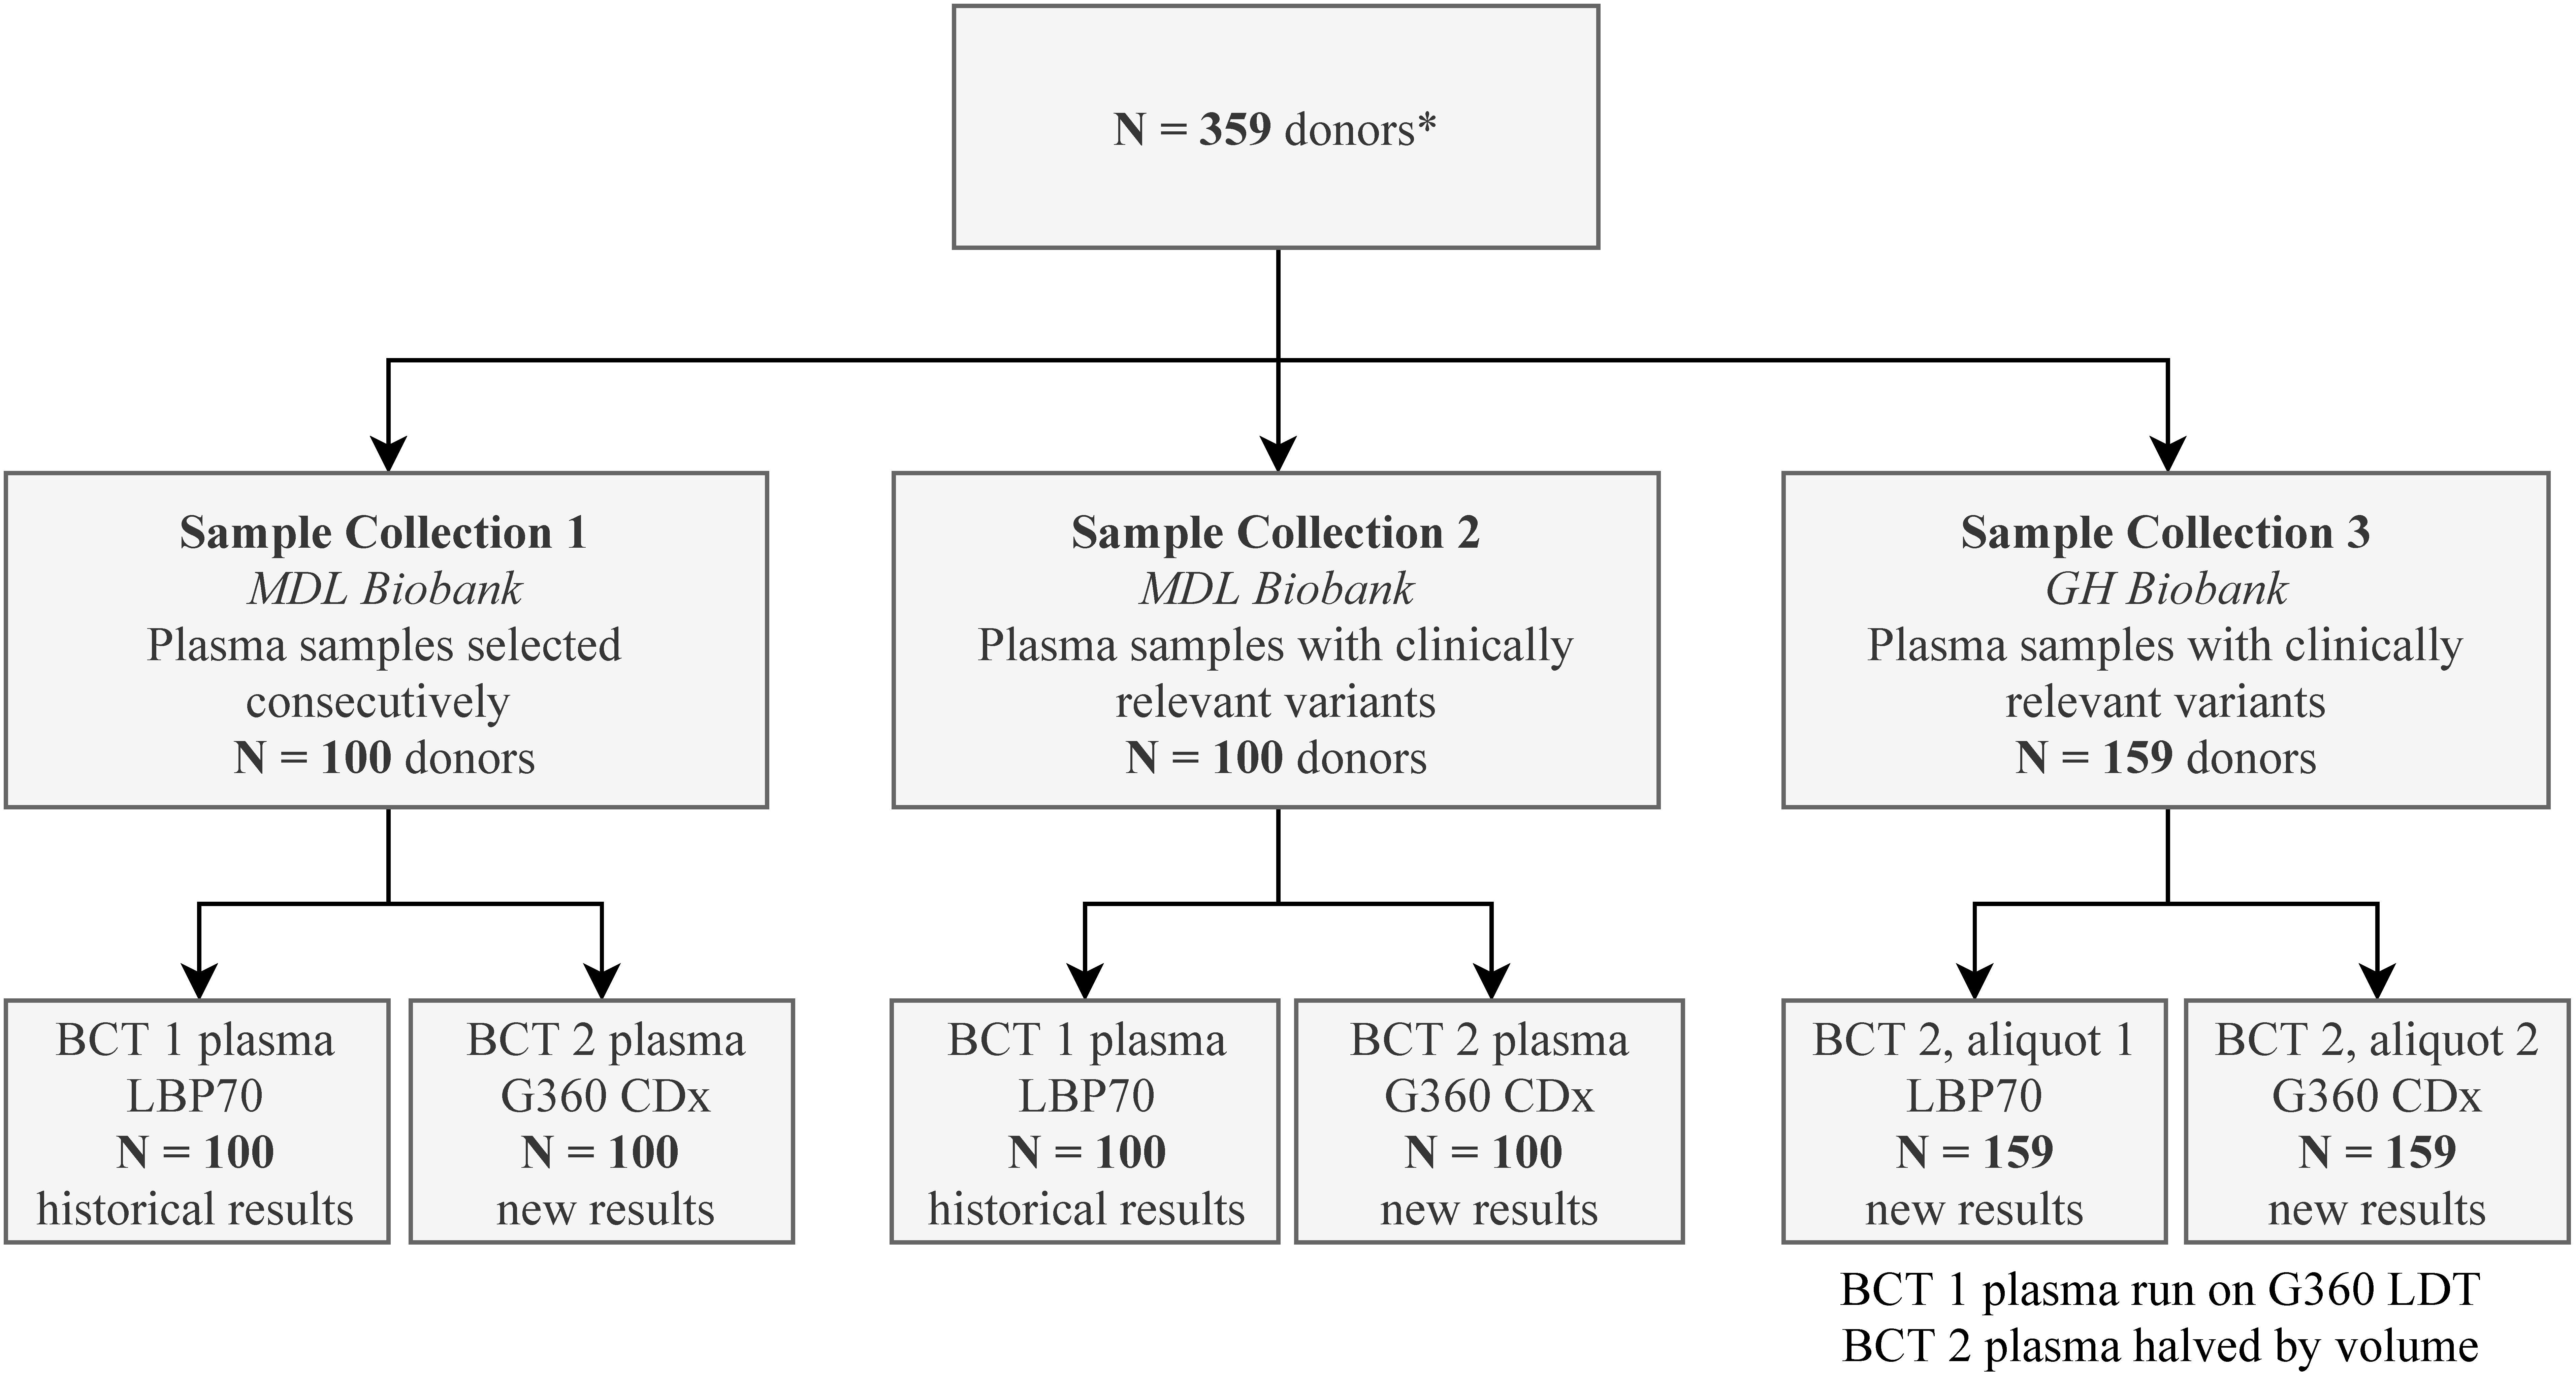
\includegraphics{figures/study_workflow.png}
    \caption{\textbf{Study Diagram}. *Sixteen and eleven donor samples were not included due to 
    instrument failures during the LBP70 and G360 CDx tests, respectively. Hence, blood was
    collected from 386 donors.}\label{f:study_diagram}
\end{figure}

\section{PROCEDURE}

\begin{enumerate}
	\item DATES OF STUDY
	    \begin{enumerate}
            \item The study was performed between NOV-11-2018 to MAR-22-2019. The samples were
                processed on G360 CDx system from NOV-27-2018 to MAR-11-2019. The samples were
                processed at MDL on LBP70 platform from NOV-11-2018 to MAR-22-2019.
	    \end{enumerate}
    \item SAMPLES
        \begin{enumerate}
            \item Samples were selected and obtained based on the protocol \textbf{D-000631,
                Section 6.1.2}. The inclusion and exclusion criteria for samples were based on
                \textbf{D-000631, Section 6.1.3}. Samples were selected in consecutive order
                regardless of MAF.
            \item The distribution of cancer types tested is provided in \cref{a:cancer_types}.
            \item Samples obtained from collection 1, 2 and 3 were accessioned at GH and processed
                on G360 CDx platform. For collection 3, 159 plasma retains were selected from GH
                biobank and were split into 2 equal aliquots, where one aliquot was run on G360 CDx
                and second aliquot on LBP70 platform at MDL. All the aliquots were accessioned at
                GH. The second aliquot was sent to MDL in 3 shipments. A detailed list of samples
                that were shipped to MDL is archived in the location provided in
                \cref{a:List_of_data_archived_on_server_and_server_locations}.               
    	\end{enumerate}
	\item MATERIALS/EQUIPMENT
    \begin{enumerate}
        \item Materials and equipment were used in accordance to \textbf{D-000631}. The storage
            locations for all manual report forms are listed in
            \cref{a:List_of_data_archived_on_server_and_server_locations}.
    	\item Reagent lots of Guardant360 CDx SPK Kits are listed in \cref{a:Guardant360_CDx_SPK_Lot_Numbers}.
    	\item Critical instruments used in this study are tabulated in \cref{t:instrument_list}.
\end{enumerate}
	
\captionsetup{justification=raggedright, singlelinecheck=off,skip=0pt}
\begin{table}[H]
\centering
\begin{threeparttable}
\caption[Critical Instrumens Used for the Study]{\textbf{Critical Instrumens Used for the Study}} \label{t:instrument_list}
\begin{tabular}{|L{3in}|L{4in}|} \hline
\rowcolor [gray]{.85} 
\textbf{Instrument Type} & 
\textbf{Internal Instrument ID (Serial Number)} \\ \hline
QIAsymphony SP Instrument (Qiagen) & QSY00003 (34718), QSY00006 (35059) \\ \hline
Microlab STARlet(Hamilton Robotics) & STL00008 (C596), STL00009 (C634) \\ \hline
Microlab STAR (Hamilton Robotics) & STA00014 (C473), STA00015 (C488) \\ \hline
Veriti 96-Well Thermal Cycler (Applied Biosystems) & TCC00046 (2990237107), 
    TCC00047 (2990237108), TCC00048 (2990237110), TCC00049 (2990237111) \\ \hline
4200 TapeStation (Agilent Technologies) & TAP00006 (DEDAA01312), 
    TAP00005 (DEDAA00939), TAP00007 (DEDAA01313) \\ \hline
NextSeq 550 Sequencing System (Illumina) & NSQ00011 (NB551146), 
    NSQ00019 (NB551346), NSQ00020 (NB551347), NSQ00021 (NB551348) \\ \hline
\end{tabular}
\end{threeparttable}
\end{table}
    
\item METHOD
	\begin{enumerate}
        \item Testing was conducted in the Guardant Health clinical laboratory located at 505
            Penobscot Drive, Redwood City, CA 94063 USA by trained clinical laboratory personnel.
            The operators are listed in \cref{a:Operator_groups_and_names}.
        \item The study was performed according to \textbf{D-000631} using the configuration as
            defined in \cref{a:Instrument_and_Software_Versions}.
        \item Library Prep to Sequencing were performed per \textbf{D-000631}, Section 9.2.2. All
            batches in the study (51, 52, 53, 54, 55, 56, 59, 61 and 1002) were processed in ACS.\@
            The data for those batches, including in-process QC metrics, equipment, and reagents,
            are maintained in ACS.\@
        \item The study was conducted in alignment with the conditions indicated in the protocol.
            See \cref{t:instrument_ids}.
	\end{enumerate}
\end{enumerate}

\captionsetup{justification=raggedright,singlelinecheck=off,skip=0pt}
\begin{table}[H]
\centering
\begin{threeparttable}
\caption{\textbf{Summary of Study Conduct}} \label{t:instrument_ids}
\begin{tabular}{|L{1.0in}|L{1in}|L{0.9in}|L{0.9in}|L{0.9in}|L{0.9in}|L{0.9in}|}
    \hline
    \rowcolor [gray]{.85} 
    \textbf{ACS Batches run consecutively on the same set of instruments}  & 
        \textbf{QIAsymphony Internal ID} & 
        \textbf{Hamilton STARlet Internal ID} & \textbf{Hamilton STAR Internal ID} & 
        \textbf{Thermal-cyclers Internal ID} & \textbf{Tape Station Internal ID} & 
        \textbf{NextSeqs: Internal ID} \\ \hline
    51 and 53 & QSY00003 & STL00008 & STA00014 & TCC00046 TCC00047 & 
        TAP00006 TAP00007 & NSQ00011 NSQ00019 \\ \hline
    52 and 54 & QSY00006 & STL00009 & STA00015 & TCC00048 TCC00049 & 
        TAP00006 TAP00007 & NSQ00020 NSQ00020 \\ \hline
    55 and 56 & QSY00006 & STL00008 & STA00014 & TCC00046 TCC00047 & 
        TAP00006 TAP00007 & NSQ00011 NSQ00019 \\ \hline
    59 and 61 & QSY00006 & STL00008 & STA00014 & TCC00048 TCC00049 & 
        TAP00006 TAP00007 & NSQ00011 NSQ00019 \\ \hline
    1002 & QSY00006 & STL00009 / STL00008 & STA00014 / STA00015 & TCC00048 TCC00049 & 
        TAP00006 TAP00005 & NSQ00020 NSQ00021\\ \hline
\end{tabular}
\end{threeparttable}
\end{table}

\captionsetup{justification=raggedright,singlelinecheck=off,skip=0pt}
\begin{table}[H]
\centering
\begin{threeparttable}
\caption[Summary of Study Conditions vs. Study Protocol]{\textbf{Summary of Study Conditions vs.
    Study Protocol}}\label{t:study_conditions_actual}
\begin{tabular}{|L{2.0in}|L{1.0in}|L{3.0in}|}
    \hline
    \rowcolor [gray]{.85}
    \textbf{Study Condition}  & 
    \textbf{Protocol (D-000631)} & 
    \textbf{Actual Numbers } \\ \hline
    Sample Size & N $\geq$ 370  & *386 donor blood collections. 
        All samples from 27 blood collections did not complete 
        due to instrument failures (\cref{f:study_diagram}). \\ \hline
    Number of Guardant360 SPK Lots & ≥ 1 & 2  \\ \hline
    Number of Testing Sites & 1 & 1 \\ \hline
    Number of Instruments & ≥ 1 & QIAsymphony (2), Hamilton-Starlet (2), 
        Hamilton-Star (2), Thermal cycler (4), Illumina NextSeq 550 (4),
        TapeStation (3) \\ \hline
    Number of Operator Groups & ≥ 2 & 6 \\ \hline
    Number of Testing on Non-Consecutive Days (as defined by run start date) & ≥ 2 & 111 \\ \hline
    Number of Consecutive Runs on the same instrument & ≥ 2 & 4 sets of 2 
        consecutive runs on the same instrument group. \\ \hline
\end{tabular}
\end{threeparttable}
\end{table}

\section{STATISTICAL ANALYSIS}

\begin{enumerate}
    \item Data analysis was performed with Python 3.5.  The location of the versioned source code
        is provided in \cref{a:List_of_data_archived_on_server_and_server_locations}.
    \item Data analysis was performed according to \textbf{D-000631, Section 10.2} except as
        described in \cref{i:not_condition} of this report.
\end{enumerate}

\section{RESULTS AND DISCUSSION}\label{s:results}

\begin{enumerate}

    \item Guardant360 CDx Results Data Set Derivation - Sample Processing and QC Metrics
	\begin{enumerate}
        \item All flowcells and variant controls in the post-screening cohort passed their
            respective sequencing QC metrics.
        \item MDL informed GH that data for the patient accessioned as SM19503665 at MDL was sent
            to GH instead of the data for patient accessioned as SM19501665 at their site.  This
            was confirmed comparing genotypes using germline variants.  All aliquots from this
            patient were excluded from analyses.
        \item Of 359 patients, no samples failed QC on G360 CDx, and three samples failed with the
            LBP70 test \cref{t:qc_table_count}.  The assay valid rates for G360 CDx and LBP70 were
            100\% and 99.2\%, respectively. Details about each QC failure are presented in
            \shortappendixref{a:qc_data}.
         \item Five samples were identified as potentially harboring germline contamination in
             the Guardant360 CDx workflow. The germline contamination metric can be confounded
             by biological factors such as the presence of another genome (e.g., from an organ
             transplant) or allele imbalance caused in high tumor fraction samples. All
             potentially contaminating germline events were determined to be due to biological
             characteristics of the patients and not from between-sample contamination, and
             they were included in the call agreement analyses (refer to the fuller explanation
             in \emph{Section 9.3} of \textbf{D-000185}).
	\end{enumerate}

\captionsetup{justification=justified,singlelinecheck=off,skip=0pt}
\begin{table}[H]
\centering
\begin{threeparttable}
\caption[Number of QC failures by the LBP70 test and G360 CDx] {\textbf{Number of QC failures by
    the LBP70 and G360 CDx tests.}}\label{t:qc_table_count}
\begin{tabular}{|l|C{1.5in}|C{1.5in}|C{1in}|}
\hline
\rowcolor[gray]{.85}\textbf{SC} & \textbf{LBP70 QC Fail, G360 CDx QC Pass} & \textbf{LBP70 QC Pass, G360 CDx QC Pass} & \textbf{  Total Samples }\\ \hline
             1 &                                0 &                              100 &            100 \\ \hline
             2 &                                0 &                              100 &            100 \\ \hline
             3 &                                3 &                              156 &            159 \\ \hline
 Total Samples &                                3 &                              356 &            359 \\ \hline
\end{tabular}
\caption*{The second column provides, for each sample collection, the  number of samples that
    failed QC metrics with the LBP70 test but not with the G360 CDx. The third column gives the
    number of samples that passed QC with the LBP70 test but failed QC with the G360 CDx.}
\end{threeparttable}
\end{table}
	
	\item Variant call agreement
	\begin{enumerate}
      \item All variant calls were retrieved according to \textbf{Sections 10.2.2.1} and
          \textbf{10.2.2.2} of \textbf{D-000631}.
      \item\label{i:manual_review} In agreement with \textbf{Section 10.3.3} of \textbf{D-000631},
          differences in variant annotations that may arise from differences (e.g., variant phasing
          differences) between bioinformatics pipelines were manually reviewed and reconciled prior
          to analysis of agreement as documented in \cref{a:reviewed_calls}, resulting in updated
          concordance status for 6 of the 302 indels (2.0\%) and 7 out of 1483 SNVs (0.47\%) called
          positive by MDL.\@
      \item NPA for SNVs and indels was evaluated at variant sites that were detected positive in
          at least one sample of the study (refer to \textbf{Section 6.2.9} of \textbf{D-000631}).
          CNVs were evaluated for negative agreement for two genes (ERBB2 and MET). Fusions were
          evaluated in four categories: gene fusions including NTRK1, RET, ROS1, and ALK.
      \item The PPA and NPA for each sample collection and variant category are shown in
          \cref{t:ppa_summary_collections_rawrawraw,t:npa_summary_collections_rawrawraw},
          respectively.
            
            \captionsetup{justification=justified,singlelinecheck=off,skip=0pt}
            \begin{table}[H]
            \centering
            \begin{threeparttable}
            \caption{\textbf{PPA, P(G360 CDx+ | LBP70 +), for each 
                sample collection and variant category.}}
            \begin{tabular}{|l|l|c|c|c|c|c|c|}
\hline
\rowcolor[gray]{.85}            &         &  \multicolumn{2}{c|}{\textbf{Collection 1}}  &  \multicolumn{2}{c|}{\textbf{Collection 2}}  &  \multicolumn{2}{c|}{\textbf{Collection 3}} \\ \hline
\rowcolor[gray]{.85}            &         & \textbf{PPA} & \textbf{n} & \textbf{PPA} & \textbf{n} & \textbf{PPA} & \textbf{    n }\\ \hline
\multirow{4}{*}{Clinically Relevant} & SNV &         91.9 &   37 &         95.0 &   80 &         92.1 &   89 \\ \cline{2-8}
           & Indel &        100.0 &    6 &         93.9 &   33 &         80.0 &   65 \\ \cline{2-8}
           & CNA &         70.0 &   10 &         88.5 &   26 &         73.9 &   23 \\ \cline{2-8}
           & Fusion &           NA &    0 &        100.0 &    3 &         97.1 &   35 \\ \hline
\multirow{2}{*}{Panel-wide} & SNV &         85.9 &  333 &         78.6 &  407 &         81.1 &  735 \\ \cline{2-8}
           & Indel &         85.7 &   42 &         86.9 &   61 &         78.1 &  192 \\ \hline
\end{tabular}
            \caption*{``n'' is the number of positives called by the LBP70 test.}
            \label{t:ppa_summary_collections_rawrawraw}
            \end{threeparttable}
            \end{table}
            
            \captionsetup{justification=justified,singlelinecheck=off,skip=0pt}
            \begin{table}[H]
            \centering
            \begin{threeparttable}
            \caption{\textbf{NPA, P(G360 CDx\textminus | LBP70\textminus), 
                for each sample collection and variant category.}}
            \label{t:npa_summary_collections_rawrawraw}
            \begin{tabular}{|l|l|c|c|c|c|c|c|}
\hline
\rowcolor[gray]{.85}            &         &  \multicolumn{2}{c|}{\textbf{Collection 1}}  &  \multicolumn{2}{c|}{\textbf{Collection 2}}  &  \multicolumn{2}{c|}{\textbf{Collection 3}} \\ \hline
\rowcolor[gray]{.85}            &         & \textbf{NPA} & \textbf{n} & \textbf{NPA} & \textbf{n} & \textbf{NPA} & \textbf{       n }\\ \hline
\multirow{4}{*}{Clinically Relevant} & SNV &       99.962 &    7963 &       99.949 &    7920 &       99.919 &   12391 \\ \cline{2-8}
           & Indel &      100.000 &    9794 &       99.990 &    9767 &       99.901 &   15223 \\ \cline{2-8}
           & CNA &       99.474 &     190 &       99.425 &     174 &       99.654 &     289 \\ \cline{2-8}
           & Fusion &      100.000 &     400 &      100.000 &     397 &       99.321 &     589 \\ \hline
\multirow{2}{*}{Panel-wide} & SNV &       99.987 &  399067 &       99.987 &  398993 &       99.978 &  622329 \\ \cline{2-8}
           & Indel &       99.992 &   75158 &       99.995 &   75139 &       99.969 &  117120 \\ \hline
\end{tabular}
            \caption*{``n''
            is the number of \textcolor{blue}{variant sites as defined in 
            Section 6.2.9 of \textbf{D-000631}. During the analysis, it was
            found that the incorrect ``n'' was used for panel-wide Indels
            in report \textbf{D-000089}. In that report, the number of evaluable
            SNV sites was applied to the Indel category as well. In the analysis for this
            report, this was corrected. The change had a very slight impact
            on panel-wide Indel NPA values which did not affect any conclusions.}}
            \end{threeparttable}
            \end{table}
            
      \item The PPA values from all sample collections were combined into overall PPA values in
          \cref{t:ppa_combined4}. The NPA values in \cref{t:npa_combined4} compared against the
          acceptance criteria were calculated from Sample Collection 1 in accordance with
          \textbf{Sections 6.2.10} and \textbf{10.4.3.4} of \textbf{D-000631}.
      \item\label{i:not_condition} In the third sample collection, it was expected that samples
          selected using G360 LDT results may have different PPA between LBP70 and Guardant360 CDx
          than an unselected set of samples. To account for this expectation, the protocol called
          for conditioning on the positive/negative status with G360 LDT testing to estimate PPA.
          However, it was found that there was no difference in agreement (PPA) levels for this
          for this sample collection versus unselected cohorts
          (\cref{a:conditional_concordance}), so the analysis continued without conditioning on
          G360 LDT results for the third sample collection as presented in
          \cref{t:ppa_combined4,t:npa_combined4}.
      
            \captionsetup{justification=justified,singlelinecheck=off,skip=0pt}
            \begin{table}[H]
            \centering
            \begin{threeparttable}
            \caption[PPA for each variant category over all samples]
            {\textbf{PPA for each variant category over all samples.}}
            \label{t:ppa_combined4}
            \begin{tabular}{|l|l|C{1.0in}|C{0.7in}|C{0.7in}|c|c|c|}
\hline
\rowcolor[gray]{.85}            &         & \textbf{Acceptable LLCI PPA} & \textbf{CDx+ LBP70+} & \textbf{CDx{\textminus} LBP70+} & \textbf{PPA} & \textbf{LLCI} & \textbf{  ULCI }\\ \hline
\multirow{4}{1in}{Clinically Relevant} & SNV &                 72.0 &          192 &                      14 &  93.2 &  88.9 &  96.2 \\ \cline{2-8}
           & Indel &                 72.0 &           89 &                      15 &  85.6 &  77.3 &  91.7 \\ \cline{2-8}
           & CNA &                 60.0 &           47 &                      12 &  79.7 &  67.2 &  89.0 \\ \cline{2-8}
           & Fusion &                 70.0 &           37 &                       1 &  97.4 &  86.2 &  99.9 \\ \hline
\multirow{2}{*}{Panel-wide} & SNV &                 74.0 &         1202 &                     273 &  81.5 &  79.4 &  83.4 \\ \cline{2-8}
           & Indel &                 76.0 &          239 &                      56 &  81.0 &  76.1 &  85.3 \\ \hline
\end{tabular}
            \caption*{The 95\% Clopper-Pearson confidence intervals are shown 
            in the LLCI and ULCI columns.}
            \end{threeparttable}
            \end{table}
            
            \captionsetup{justification=justified,singlelinecheck=off,skip=0pt}
            \begin{table}[H]
            \centering
            \begin{threeparttable}
            \caption{\textbf{NPA for Sample Collection 1.}}
            \label{t:npa_combined4}
            \begin{tabular}{|l|l|C{1.0in}|C{0.7in}|C{0.7in}|c|c|c|}
\hline
\rowcolor[gray]{.85}            &         & \textbf{Acceptable LLCI NPA} & \textbf{CDx+ LBP70{\textminus}} & \textbf{CDx{\textminus} LBP70{\textminus}} & \textbf{NPA} & \textbf{LLCI} & \textbf{     ULCI }\\ \hline
\multirow{4}{1in}{Clinically Relevant} & SNV &                 99.6 &                       3 &                               7960 &   99.962 &  99.890 &   99.992 \\ \cline{2-8}
           & Indel &                 99.8 &                       0 &                               9794 &  100.000 &  99.962 &  100.000 \\ \cline{2-8}
           & CNA &                 88.0 &                       1 &                                189 &   99.474 &  97.103 &   99.987 \\ \cline{2-8}
           & Fusion &                 98.0 &                       0 &                                400 &  100.000 &  99.082 &  100.000 \\ \hline
\multirow{2}{*}{Panel-wide} & SNV &                 99.9 &                      50 &                             399017 &   99.987 &  99.983 &   99.991 \\ \cline{2-8}
           & Indel &                 99.9 &                       6 &                              75152 &   99.992 &  99.983 &   99.997 \\ \hline
\end{tabular}
            \caption*{The 95\% Clopper-Pearson confidence intervals are 
            shown in the LLCI and ULCI columns.}
            \end{threeparttable}
            \end{table}
                    
        \item The PPA and NPA for all samples for each of the clinically significant 
              variant categories over all sample collections
              are shown in \cref{t:coll4_variant_classspecial_raw_binomial_2test}.
              Tables with the number of concordant and discordant calls for each sample
	          collection for each clinically relevant variant category
	          are in \cref{a:call_concordance_tables_raw}.
	   
        \captionsetup{justification=justified,singlelinecheck=off,skip=0pt}
        \begin{table}[H]
        \centering
        \begin{threeparttable}
        \caption[PPA and NPA for each variant class over all sample collections]
        {\textbf{PPA and NPA for each variant class over all sample collections.}}
        \label{t:coll4_variant_classspecial_raw_binomial_2test}
        \scriptsize
        \begin{tabular}{|l|C{0.54in}|C{0.54in}|C{0.54in}|C{0.54in}|c|c|}
\hline
\rowcolor[gray]{.85}{}                           & \textbf{CDx+ LBP70+} & \textbf{CDx{\textminus} LBP70+} & \textbf{CDx+ LBP70{\textminus}} & \textbf{CDx{\textminus} LBP70{\textminus}} & \textbf{PPA} & \textbf{                                       NPA }\\ \hline
BRAF Activating SNV         &           21 &                       0 &                       1 &                                334 &  \makecell{100.0 \\ (83.9 - 100.0)} &    \makecell{99.701 \\ (98.348 - 99.992)} \\ \hline
BRCA1 Inactivating SNV      &           15 &                       2 &                       5 &                              10302 &    \makecell{88.2 \\ (63.6 - 98.5)} &    \makecell{99.951 \\ (99.887 - 99.984)} \\ \hline
BRCA2 Inactivating SNV      &           12 &                       1 &                       0 &                               6395 &    \makecell{92.3 \\ (64.0 - 99.8)} &  \makecell{100.000 \\ (99.942 - 100.000)} \\ \hline
EGFR L858R                  &           18 &                       0 &                       1 &                                337 &  \makecell{100.0 \\ (81.5 - 100.0)} &    \makecell{99.704 \\ (98.363 - 99.993)} \\ \hline
EGFR T790M                  &           19 &                       1 &                       3 &                                333 &    \makecell{95.0 \\ (75.1 - 99.9)} &    \makecell{99.107 \\ (97.413 - 99.815)} \\ \hline
KRAS Activating SNVs        &           60 &                       6 &                       4 &                               4558 &    \makecell{90.9 \\ (81.3 - 96.6)} &    \makecell{99.912 \\ (99.776 - 99.976)} \\ \hline
NRAS Activating SNVs        &           28 &                       3 &                       3 &                               3882 &    \makecell{90.3 \\ (74.2 - 98.0)} &    \makecell{99.923 \\ (99.774 - 99.984)} \\ \hline
Other EGFR activating SNVs  &           19 &                       1 &                       0 &                               2116 &    \makecell{95.0 \\ (75.1 - 99.9)} &  \makecell{100.000 \\ (99.826 - 100.000)} \\ \hline
BRCA2 Inactivating Indel    &           27 &                       9 &                      11 &                              19889 &    \makecell{75.0 \\ (57.8 - 87.9)} &    \makecell{99.945 \\ (99.901 - 99.972)} \\ \hline
BRCA1 Inactivating Indel    &           13 &                       5 &                       4 &                               7810 &    \makecell{72.2 \\ (46.5 - 90.3)} &    \makecell{99.949 \\ (99.869 - 99.986)} \\ \hline
EGFR Activating Indel       &           31 &                       1 &                       1 &                               2815 &    \makecell{96.9 \\ (83.8 - 99.9)} &    \makecell{99.964 \\ (99.802 - 99.999)} \\ \hline
ERBB2 Activating Indel      &           11 &                       0 &                       0 &                               1057 &  \makecell{100.0 \\ (71.5 - 100.0)} &  \makecell{100.000 \\ (99.652 - 100.000)} \\ \hline
Other EGFR activating Indel &            7 &                       0 &                       0 &                               3197 &  \makecell{100.0 \\ (59.0 - 100.0)} &  \makecell{100.000 \\ (99.885 - 100.000)} \\ \hline
Homopolymer                 &           54 &                      13 &                       7 &                              86078 &    \makecell{80.6 \\ (69.1 - 89.2)} &    \makecell{99.992 \\ (99.983 - 99.997)} \\ \hline
Long Indel                  &           10 &                       4 &                       4 &                               8882 &    \makecell{71.4 \\ (41.9 - 91.6)} &    \makecell{99.955 \\ (99.885 - 99.988)} \\ \hline
ERBB2 Amplification         &           20 &                       2 &                       0 &                                334 &    \makecell{90.9 \\ (70.8 - 98.9)} &  \makecell{100.000 \\ (98.902 - 100.000)} \\ \hline
MET Amplification           &           27 &                      10 &                       3 &                                316 &    \makecell{73.0 \\ (55.9 - 86.2)} &    \makecell{99.060 \\ (97.276 - 99.806)} \\ \hline
NTRK1 Fusion                &            5 &                       0 &                       0 &                                351 &  \makecell{100.0 \\ (47.8 - 100.0)} &  \makecell{100.000 \\ (98.955 - 100.000)} \\ \hline
RET Fusion                  &           11 &                       1 &                       2 &                               1410 &    \makecell{91.7 \\ (61.5 - 99.8)} &    \makecell{99.858 \\ (99.489 - 99.983)} \\ \hline
ROS1 Fusion                 &           11 &                       0 &                       0 &                               1413 &  \makecell{100.0 \\ (71.5 - 100.0)} &  \makecell{100.000 \\ (99.739 - 100.000)} \\ \hline
ALK Fusion                  &           10 &                       0 &                       2 &                                344 &  \makecell{100.0 \\ (69.2 - 100.0)} &    \makecell{99.422 \\ (97.928 - 99.930)} \\ \hline
\end{tabular}
        \caption*{ The 95\% Clopper-Pearson confidence intervals are shown in parantheses.
            ``Homopolymer'' refers to indels adjacent to a homopolymeric five or more identical
            nucleotides, a homopolymeric sequence (\textbf{D-000631, section 6.1.5.2.2}).  ``Long
            indel'' refers to indels greater than 30 base pairs (\textbf{D-000631, Section
            6.1.5.2.1}). Samples were selected such that each variant class had ten G360 LDT
            positives (\textbf{D-000631, section 6.1.5.1}).  Some rows may have fewer than ten
            positive samples when both G360 CDx and the LBP70 test did not detect G360 LDT-positive
            samples.}
        \end{threeparttable}
        \end{table}
        \item Lower concordance and PPA observed for BRCA1 / BRCA2 inactivating frameshift indels
            is explained by five samples with a primary activating germline BRCA2 alteration and
            multiple reversion mutations that restore the reading frame arising as a resistance
            mechanism. This represents a commonly documented pattern of resistence, where
            subclonally many distinct mutations arise independently to compensate for the primary
            frame shift in unique ways in order to restore the reading frame and obtain a
            functional BRCA protein. Such mutations typically arise at very low-MAF levels
            representing multiple independent subclones of resistance. In these patients, actual
            primary inactivating mutations were all detected concordantly. Moreover, for each
            patient of this type, both LBP70 and G360 CDx tests detected reversion mutations
            representing the same biological phenomenon and accurately representing patient state
            with respect to the reading frame of the protein, yet the mutations detected were
            sometimes distinct due to stochastic detection of low allele frequency events. So,
            overall PPA for this category of variants was lower than one would expect for
            clinically significant drivers since many represented non-driver subclonal resistance
            mutations. Important, patient status with respect to reversion was concordantly
            detected by both tests in all patients
    
    \end{enumerate}
	
    \item Concordance for focal CNAs

	\begin{enumerate}
      \item G360 CDx only reports focal CNAs. It does not report CNA calls for which the
          surrounding genes on the same chromosome arm are also amplified at a similar level. The
          LBP70 test reports all detected amplifications, focal or not. Of the 31 focal CNAs
          reported by G360 CDx, 28 were reported by the LBP70 test (PPV = 90.3\% with a 95\%
          exact confidence interval of 74.2\% to 98.0\%).
    \end{enumerate}
    
    \color{blue}
    \item Data analysis for restricted reportable range (55 genes)
    \begin{enumerate}
        \item As described in Section 10.4.10 of \textbf{D-000631}, the analysis to produce
            \cref{t:ppa_combined4,t:npa_combined4} was repeated but only for variants in the
            restricted reportable range implemented in BIP 3.5.3.
        
        \item The original line data attached to report \textbf{D-000089} was used
        	as input to the analysis to reproduce all previous tables. The line
        	data attached to this report, \textbf{D-000632}, was used to generate
        	the PPA and NPA values from the restricted reportable range
        	implemented in BIP 3.5.3 (\cref{t:PPA_combined_bips,t:PPA_combined_bips}). 
        
        \item \cref{t:PPA_combined_bips} presents a comparison of PPA values 
        	using the larger reportable range analyzed in 
       		\cref{t:ppa_combined4} versus the
       		restricted reportable range. \cref{t:PPA_combined_bips} presents
       		the same comparison for NPA values.
            
        \captionsetup{justification=justified,singlelinecheck=off,skip=0pt}
        \begin{table}[H]
        \color{blue}
        \centering
        \begin{threeparttable}
        \caption{\textbf{PPA for each variant category over all samples using reportable range
            implemented in BIP 3.5.3.}}
        \label{t:PPA_combined_bips}
        \begin{tabular}{|l|l|L{1.0in}|L{0.5in}|C{0.7in}|C{0.7in}|c|c|c|}
\hline
\rowcolor[gray]{.85}{}  &  {}  & \textbf{Acceptable LLCI PPA} & \textbf{BIP} & \textbf{CDx+ LBP70+} & \textbf{CDx{\textminus} LBP70+} & \textbf{PPA} & \textbf{LLCI} & \textbf{  ULCI }\\ \hline
\multirow{8}{0.75in}{Clinically Relevant} & \multirow{2}{*}{SNV} & \multirow{2}{*}{72.0} & 3.5.2 &          192 &                      14 &  93.2 &  88.9 &  96.2 \\ \cline{4-9}
           &       &      & 3.5.3 &          192 &                      14 &  93.2 &  88.9 &  96.2 \\ \cline{2-9}
           & \multirow{2}{*}{Indel} & \multirow{2}{*}{72.0} & 3.5.2 &           89 &                      15 &  85.6 &  77.3 &  91.7 \\ \cline{4-9}
           &       &      & 3.5.3 &           88 &                      15 &  85.4 &  77.1 &  91.6 \\ \cline{2-9}
           & \multirow{2}{*}{CNA} & \multirow{2}{*}{60.0} & 3.5.2 &           47 &                      12 &  79.7 &  67.2 &  89.0 \\ \cline{4-9}
           &       &      & 3.5.3 &           47 &                      12 &  79.7 &  67.2 &  89.0 \\ \cline{2-9}
           & \multirow{2}{*}{Fusion} & \multirow{2}{*}{70.0} & 3.5.2 &           37 &                       1 &  97.4 &  86.2 &  99.9 \\ \cline{4-9}
           &       &      & 3.5.3 &           37 &                       1 &  97.4 &  86.2 &  99.9 \\ \hline
\multirow{4}{0.75in}{Panel-wide} & \multirow{2}{*}{SNV} & \multirow{2}{*}{74.0} & 3.5.2 &         1202 &                     273 &  81.5 &  79.4 &  83.4 \\ \cline{4-9}
           &       &      & 3.5.3 &          436 &                      40 &  91.6 &  88.7 &  93.9 \\ \cline{2-9}
           & \multirow{2}{*}{Indel} & \multirow{2}{*}{76.0} & 3.5.2 &          239 &                      56 &  81.0 &  76.1 &  85.3 \\ \cline{4-9}
           &       &      & 3.5.3 &          126 &                      25 &  83.4 &  76.5 &  89.0 \\ \hline
\end{tabular}
        \caption*{The 95\% Clopper-Pearson confidence intervals are shown 
        in the LLCI and ULCI columns.}
        \end{threeparttable}
        \end{table}
        
        \captionsetup{justification=justified,singlelinecheck=off,skip=0pt}
        \begin{table}[H]
        \color{blue}
        \centering
        \begin{threeparttable}
        \caption{\textbf{NPA for Sample Collection 1 using reportable range implemented in BIP
            3.5.3.}}
        \label{t:npa_combined4_rrr}
        \begin{tabular}{|l|l|L{1.0in}|L{0.5in}|C{0.7in}|C{0.7in}|c|c|c|}
\hline
\rowcolor[gray]{.85}{}  &  {}  & \textbf{Acceptable LLCI NPA} & \textbf{BIP} & \textbf{CDx+ LBP70{\textminus}} & \textbf{CDx{\textminus} LBP70{\textminus}} & \textbf{NPA} & \textbf{LLCI} & \textbf{     ULCI }\\ \hline
\multirow{8}{0.75in}{Clinically Relevant} & \multirow{2}{*}{SNV} & \multirow{2}{*}{99.6} & 3.5.2 &                       3 &                               7960 &   99.962 &   99.890 &   99.992 \\ \cline{4-9}
           &       &      & 3.5.3 &                       3 &                               7660 &   99.961 &   99.886 &   99.992 \\ \cline{2-9}
           & \multirow{2}{*}{Indel} & \multirow{2}{*}{99.8} & 3.5.2 &                       0 &                               9794 &  100.000 &   99.962 &  100.000 \\ \cline{4-9}
           &       &      & 3.5.3 &                       0 &                               9394 &  100.000 &   99.961 &  100.000 \\ \cline{2-9}
           & \multirow{2}{*}{CNA} & \multirow{2}{*}{88.0} & 3.5.2 &                       1 &                                189 &   99.474 &   97.103 &   99.987 \\ \cline{4-9}
           &       &      & 3.5.3 &                       1 &                                189 &   99.474 &   97.103 &   99.987 \\ \cline{2-9}
           & \multirow{2}{*}{Fusion} & \multirow{2}{*}{98.0} & 3.5.2 &                       0 &                                400 &  100.000 &   99.082 &  100.000 \\ \cline{4-9}
           &       &      & 3.5.3 &                       0 &                                400 &  100.000 &   99.082 &  100.000 \\ \hline
\multirow{4}{0.75in}{Panel-wide} & \multirow{2}{*}{SNV} & \multirow{2}{*}{99.9} & 3.5.2 &                      50 &                             399017 &   99.987 &   99.983 &   99.991 \\ \cline{4-9}
           &       &      & 3.5.3 &                      10 &                            3855876 &  100.000 &  100.000 &  100.000 \\ \cline{2-9}
           & \multirow{2}{*}{Indel} & \multirow{2}{*}{99.9} & 3.5.2 &                       6 &                              75152 &   99.992 &   99.983 &   99.997 \\ \cline{4-9}
           &       &      & 3.5.3 &                       0 &                            4414987 &  100.000 &  100.000 &  100.000 \\ \hline
\end{tabular}
        \caption*{The 95\% Clopper-Pearson confidence intervals are 
        shown in the LLCI and ULCI columns.}
        \end{threeparttable}
        \end{table}
        


    \end{enumerate}


     
  
  	 \color{black}
     \item Deviations
   	 \begin{enumerate}
        \item NER-2018-0488: Flowcell H3GCMBGX9 was loaded on sequencer NSQ00021; however, the run
            was aborted due to a hardware failure. The batch was re-enriched in accordance to
             SOP-TDV-000071, and the affected samples were loaded onto a new flowcell, HKHTKBGX7,
             and sequenced on NSQ00020.
        \item NER-2019-0103: On 11/29/2018, shortly after loading flowcell H3GCMBGX9, NextSeq
            NSQ00021 encountered a Hardware Error. The instrument was taken out-of-service for
             repair.  Refer to NER-2018-0488 above.
        \item NER-2019-0030: The temperature of freezer FZR00048 fell out of the acceptable range
            (\textminus80\textdegree{}C~\textpm~10 \textdegree{}C) for more than three hours. All
             plasma samples were transferred to another qualified freezer (FZR00070). There was no
             observed impact since all affected samples passed in-process QC metrics.
        \item NER-2019-0233: During the execution of the study, two independent
            events resulted in batch failures. The first event occurred on 01/30/2019 at MD
            Anderson Clinical Laboratory (MDL) where 16 samples, sent by Guardant Health, were
            failed due to instrument failure during library preparation. In order to replace the
            samples, MDL sent 11 samples to GH for testing on the G360 CDx. These samples were
            processed on 03/11/2019 at GH, but they were not able to complete processing because
            of an instrument failure caused by a communitywide electrical power outage (PG\&E) and
            subsequent generator failure. These samples are not included in any analyses in this
            report.
        \item NER-2019-0174: Step 10.11.1.5 of SOP-TDV-000048 called for the mixing of the samples
            5-10 times using a multichannel pipette prior to transferring to a quantitation plate.
            However, it was discovered that not all of the clinical operators performed the step
            as described in the SOP.\@ The impact of not mixing the sample before transferring to
            the quantitation plate was minimal as no quantitation issue was observed in any of the
            batches.
   	\end{enumerate}
\end{enumerate}

\section{CONCLUSION}

\begin{enumerate}
    \item Of the 359 samples processed with LBP70 and Guardant360 CDx assays, three failed QC with
        the LBP70 test but not with G360 CDx. After removing the three failed samples, 356 samples
        were available for analysis.
    \item The PPA and NPA values for all six variant categories (panel-wide SNVs and Indels and
        clinically relevant SNVs, Indels, fusions, and CNA) had an acceptable agreement
        (\cref{t:ppa_combined4,t:npa_combined4}).
       	\textcolor{blue}{The panel-wide PPA and NPA for the reduced reportable range 
       	implemented in BIP 3.5.3 were higher than the larger panel with BIP 3.5.2
       	(\cref{t:ppa_combined4_rrr,t:npa_combined4_rrr}).}
    \item Guardant360 CDx is determined to be accurate as compared to the LBP70 comparator method.
\end{enumerate}

\section{APPENDICES}

\begin{itemize}
    \item \appendixref{a:List_of_data_archived_on_server_and_server_locations}
    \item \appendixref{a:Guardant360_CDx_SPK_Lot_Numbers}
    \item \appendixref{a:Operator_groups_and_names}
    \item \appendixref{a:Instrument_and_Software_Versions}
    \item \appendixref{a:cancer_types}
    \item \appendixref{a:focal_cnvs}
    \item \appendixref{a:reviewed_calls}
    \item \appendixref{a:qc_data}
    \item \appendixref{a:call_concordance_tables_raw}
    \item \appendixref{a:conditional_concordance}
\end{itemize}

\section{ATTACHMENTS}

\begin{enumerate}
    \item \texttt{Attachment 1. Line Data} 
\end{enumerate}
\newpage % Each appendix should be on a new page

%%%%%%%%%%%%%%%%%%%%%%%%% BEGIN APPENDICES %%%%%%%%%%%%%%%%%%%%%%%%%%%%%%%%%%%%%%%%%

% Change the section title format for appendices
\titleformat{\section}{\bfseries\centering}{APPENDIX~\thesection .}{3pt}{\MakeUppercase}
\begin{appendices}
\crefalias{section}{appsec}
\renewcommand{\thesection}{\arabic{section}} 

\section{List of data archived on server and server locations}
\label{a:List_of_data_archived_on_server_and_server_locations}

\begin{tabular}{|L{2in}|L{5.4in}|}
    \hline
    \rowcolor [gray]{.85} \textbf{Category} & \textbf{Type} \\ \hline
    Manual Workflow Report Forms & /ghds/ivd/analytical\_validation/D\_000089/Guardant360 CDx Processing Manual Workflow Report.pdf \\ \hline 
    Source Code used for the analysis & https://github.com/guardant/data\_science/tree/
    4812e7bbf7222e9207d0a833eb371116b0186414/08\_FDA/G360/ 180801\_ANALYTICAL\_VALIDATION/D000631 \\ \hline
    Raw sequencing data locations & The locations for 
    all of the raw data files are given in the ``Raw Sequencing Data Folder''
    column in the attached line data. As planned, raw sequencing data was not
    provided to GH for LBP70 results. \\ \hline
    BIP 3.5.3 (3.5.3-0-g8857b98) processed data locations & The locations for 
    all of the processed data files are given in the ``Sequencing Data Folder''
    column in the attached line data. \\ \hline
\end{tabular}
\clearpage


\section{Guardant360 CDx SPK Lot Numbers}
\label{a:Guardant360_CDx_SPK_Lot_Numbers}
\begin{tabular}{|L{1.4in}|L{1.3in}|L{1.3in}|L{1.3in}|L{1.3in}|}
\hline
    \rowcolor [gray]{.85} \textbf{G360 CDx SPK Lot Combination\#} & 
    \textbf{G360 CDx SPK Box 1 Lot\#} & \textbf{G360 CDx SPK Box 2 Lot\#} & 
    \textbf{G360 CDx SPK Box 3 Lot\#} & \textbf{G360 CDx SPK Box 4a-c Lot\#}\\ \hline
    SPK ``Lot A'' & 20181019A & 20181019A & 20181019A & 20181019A \\ \hline
    SPK ``Lot B'' & 000000002 & 000000007 & 000000003 & 000000008 \\ \hline
\end{tabular}
\clearpage

\section{Operator Groups and Names}
\label{a:Operator_groups_and_names}
\begin{center}
\begin{tabular}{|c|c|c|}
\hline
\rowcolor[gray] {0.85} \textbf{Operator Group} & 
    \textbf{Operator's Initial} & \textbf{Operator's Full Name} \\ \hline
OG-A & JXL , KT & JXL = Jason Loung \\ \hline
OG-B & JXL , YL, LMS & KT = Kim Phu-Ton \\ \hline
OG-C & YL , LMS, KT & LMS = Lai Mun Siew \\ \hline
OG-D & JXL, YL, LMS, KT & YL = Yesenia Lara \\ \hline
OG-E & JXL , LMS , KT  & JAL = Joyce Ann Lozano \\ \hline
OG-F & JXL , KT, JAL & TBU \\ \hline
\end {tabular}
\end{center}
\clearpage

\newpage
\section{Instrument and Software Versions}
\label{a:Instrument_and_Software_Versions}
\begin {tabular}{|L{3.5in}|L{3.5in}|}
\hline
\rowcolor[gray] {0.85} \textbf{Component} & \textbf{Version} \\ \hline
\multicolumn{2}{|l|}{\textbf{Software}}  \\ \hline
ACS & Version-v2.0-IUO-13-gf7c6d65 \\ \hline
BIP* & 3.5.2-rc2-0-g9e05762 \\ \hline
BIP-Apps & v5.0-bb8bbf9 \\ \hline
\multicolumn{2}{|l|}{\textbf{QIAsymphony}}  \\ \hline
Firmware & 4.0.3.3 \\ \hline
Management Console Software & 4.0 \\ \hline
\multicolumn{2}{|l|}{\textbf{Agilent TapeStation}}  \\ \hline
Run Controller Software & A.02.01SR1 \\ \hline
Analysis Software & A.02.01SR1 \\ \hline
\multicolumn{2}{|l|}{\textbf{Hamilton}} \\ \hline
STAR/STARlet: Venus Software & Venus Two, version 4.3.5.4785 + Service Pack 1 \\
STAR/STARlet: HHS Library & 4.4 \\ \hline
STAR/STARlet: Solid-Liquid Waste Sensor & 1.3 \\ \hline
STAR/STARlet: PX 1000uL Channel Firmware & 3.8d \\ \hline
Methods & G360\_EX\_Dilution\_v2\_7\_0, G360\_LP\_Build\_v2\_7\_0, 
G360\_LP\_Cleanup\_v2\_7\_0, G360\_EN\_Cleanup\_v2\_7\_0, 
G360\_EN\_Wash\_v2\_7\_0, G360\_AutoPooling\_v2\_7\_0 \\ \hline
Capper Decapper: Software & 1.0.2 \\ \hline
\multicolumn{2}{|l|}{\textbf{Veriti Thermocycler}} \\ \hline
Firmware & 1.7.1 \\ \hline
Protocols & LP\_PCR\_G360\_v1, ENS\_BAIT\_G360\_v1, ENS\_HYB\_G360\_v1, ENW\_PCR\_G360\_v1\\ \hline
\multicolumn{2}{|l|}{\textbf{Illumina NextSeq550}} \\ \hline
Control Software & 2.1.0 \\ \hline
RTA Software & 2.4.11 \\ \hline
Recipie Fragment & 2.1.2.1 \\ \hline
FPGA Fragment & 3.16 \\ \hline
\end{tabular}
\clearpage

\newpage
\section{Cancer Types Tested}
\label{a:cancer_types}

\captionsetup{width=0.5\textwidth}
\begin{table}[H]
    \centering
    \caption{\textbf{Distribution of cancer types tested in this study}}
    \label{t:cancer_types}
    \begin{tabular}{|l|c|}
\hline
\rowcolor[gray]{.85}\textbf{Cancer Type} & \textbf{    n }\\ \hline
             Lung &  178 \\ \hline
 Gastrointestinal &   82 \\ \hline
            Colon &   25 \\ \hline
           Breast &   17 \\ \hline
    Head and Neck &   13 \\ \hline
         Prostate &   12 \\ \hline
    Genitourinary &    7 \\ \hline
            Other &    5 \\ \hline
          Bladder &    3 \\ \hline
         Pancreas &    3 \\ \hline
          Stomach &    3 \\ \hline
            Liver &    2 \\ \hline
            Ovary &    2 \\ \hline
        Endocrine &    2 \\ \hline
           Kidney &    2 \\ \hline
      Gynocelogic &    1 \\ \hline
        Esophagus &    1 \\ \hline
             Skin &    1 \\ \hline
\end{tabular}
\end{table}
\clearpage

% \newpage
% \section{Concordance tables for focal CNAs}
% \label{a:focal_cnvs}
% 
% \captionsetup{justification=justified,singlelinecheck=off,skip=0pt}
% \begin{table}[H]
% \centering
% \begin{threeparttable}
% \caption{\textbf{CNA status for nonfocal MET CNAs detected by G360 CDx.}}
% \label{t:nonfocal_cnvs_MET}
% \begin{tabular}{|l|c|c|c|c|c|c|c|c|}
\hline
\rowcolor[gray]{.85}\textbf{Patient} &  \multicolumn{2}{c|}{\textbf{BRAF}}  &  \multicolumn{2}{c|}{\textbf{CDK6}}  &  \multicolumn{2}{c|}{\textbf{EGFR}}  &  \multicolumn{2}{c|}{\textbf{MET}} \\ \hline
\rowcolor[gray]{.85}           & \textbf{G360 CDx} & \textbf{LBP70} & \textbf{G360 CDx} & \textbf{LBP70} & \textbf{G360 CDx} & \textbf{LBP70} & \textbf{G360 CDx} & \textbf{       LBP70 }\\ \hline
 A0132526 &           F &  \textminus &  \textminus &           + &           D &  \textminus &        D &  \textminus \\ \hline
 A0132529 &           F &  \textminus &           D &  \textminus &           D &  \textminus &        D &  \textminus \\ \hline
 A0132534 &           D &           + &           D &           + &           D &           + &        D &           + \\ \hline
 A0132589 &           D &  \textminus &  \textminus &  \textminus &  \textminus &  \textminus &        D &  \textminus \\ \hline
 A0132600 &           D &  \textminus &  \textminus &           + &           D &  \textminus &        D &  \textminus \\ \hline
 A0132602 &           D &  \textminus &  \textminus &  \textminus &           D &           + &        D &  \textminus \\ \hline
 A0132619 &           F &  \textminus &           D &  \textminus &           D &           + &        D &  \textminus \\ \hline
 A0132641 &           F &           + &           D &           + &           D &           + &        D &           + \\ \hline
 A0132717 &           F &           + &  \textminus &           + &  \textminus &  \textminus &        D &           + \\ \hline
 A0132806 &           D &           + &           D &           + &           D &           + &        D &           + \\ \hline
 A0132811 &           D &           + &           D &           + &           D &           + &        D &           + \\ \hline
 A0132815 &           D &           + &           F &           + &  \textminus &  \textminus &        D &  \textminus \\ \hline
 A0132826 &           D &           + &           D &           + &           D &           + &        D &  \textminus \\ \hline
 A0132830 &           D &           + &           D &           + &           D &           + &        D &           + \\ \hline
 A0132839 &           F &  \textminus &  \textminus &  \textminus &  \textminus &  \textminus &        D &  \textminus \\ \hline
 A0132849 &           D &           + &           D &           + &           D &           + &        D &           + \\ \hline
 A0132873 &           D &  \textminus &  \textminus &  \textminus &  \textminus &  \textminus &        D &  \textminus \\ \hline
 A0133608 &  \textminus &  \textminus &  \textminus &  \textminus &           D &           + &        D &  \textminus \\ \hline
 A0133630 &  \textminus &  \textminus &           F &           + &           D &           + &        D &           + \\ \hline
 A0133876 &           D &           + &           D &           + &           D &  \textminus &        D &           + \\ \hline
 A0133879 &           D &           + &           D &           + &           D &           + &        D &           + \\ \hline
 A0133906 &           F &  \textminus &  \textminus &  \textminus &           D &  \textminus &        D &  \textminus \\ \hline
 A0133917 &           F &           + &           D &           + &           D &           + &        D &           + \\ \hline
 A0133918 &           D &  \textminus &  \textminus &  \textminus &  \textminus &  \textminus &        D &           + \\ \hline
 A0133930 &           F &           + &           D &           + &           D &           + &        D &           + \\ \hline
 A0133948 &           D &  \textminus &  \textminus &  \textminus &           D &           + &        D &  \textminus \\ \hline
 A0142194 &           D &           + &           F &           + &           D &           + &        D &           + \\ \hline
 A0142197 &           D &  \textminus &           D &  \textminus &           D &  \textminus &        D &  \textminus \\ \hline
\end{tabular}
% \caption*{
% The table shows the CNA calls for all genes on the same chromosome as MET. For
% G360 CDx, ``F'' indicates a focal CNA, ``D'' indicates a detected CNA with
% insufficient evidence
% for a focal call, and ``\textminus'' indicates that no CNA was detected. For the 
% LBP70 test, ``+'' indicates that a CNA was detected, and ``\textminus'' indicates
% that a CNA was not detected. Note that additional genes in the panel on 
% chromosome 7 (\emph{IMPDH1}, \emph{SMO}, \emph{EZH2}, and \emph{REB}) 
% were also used to determine if a CNA was focal or not, but
% the raw data was not available for the LBP70 test.}
% \end{threeparttable}
% \end{table}
% 
% \captionsetup{width=.6\textwidth,singlelinecheck=off,skip=0pt}
% \begin{table}[H]
% \centering
% \caption{\textbf{CNA status for nonfocal ERBB2 CNAs detected by G360 CDx.}}
% \label{t:nonfocal_cnvs_ERBB2}
% \begin{tabular}{|l|c|c|}
\hline
\rowcolor[gray]{.85}\textbf{Patient} &  \multicolumn{2}{c|}{\textbf{ERBB2}} \\ \hline
\rowcolor[gray]{.85}           & \textbf{G360 CDx} & \textbf{       LBP70 }\\ \hline
 A0132577 &        D &           + \\ \hline
 A0132826 &        D &           + \\ \hline
 A0132828 &        D &  \textminus \\ \hline
 A0133861 &        D &           + \\ \hline
 A0133906 &        D &  \textminus \\ \hline
 A0133913 &        D &  \textminus \\ \hline
 A0133914 &        D &           + \\ \hline
 A0133976 &        D &           + \\ \hline
 A0134012 &        D &  \textminus \\ \hline
\end{tabular}
% \caption*{Note that additional genes in the panel on 
% chromosome 17 (\emph{NF1}, \emph{CDK12}, \emph{BRCA1}, \emph{XYLT2},
% \emph{TP53}, and \emph{CHD3}) 
% were also used to determine if a CNA was focal or not, but
% the raw data was not available for the LBP70 test.}
% \end{table}

\newpage
\section{Review of variant call discordances due to BIP annotation differences}
\label{a:reviewed_calls}

As referenced in \cref{i:manual_review}, some mutations were expected
to have differences in annotation due to the different versions of the
bioinformatics pipelines run by the LBP70 test and G360 CDx.
The G360 CDx sequencing data (the ``pileups'') for all discordant indels
were investigated to identify such variants. The raw sequencing data
from the LBP70 test was not available as planned.
These revieweed calls
are listed in \cref{t:reviewed_calls}.

\captionsetup{justification=justified,singlelinecheck=off,skip=0pt}
\begin{table}[H]
\centering
\begin{threeparttable}
\caption[Review of variant call discordances due to BIP versions]
{\textbf{Review of variant call discordances due to BIP versions.}}
\label{t:reviewed_calls}
\begin{tabular}{|L{1.1in}|l|l|l|l|L{1.6in}|l|l|}
\hline
\rowcolor[gray]{.85}\textbf{Reason} & \textbf{Patient} & \textbf{Type} & \textbf{Gene} & \textbf{Position} & \textbf{Mutation} & \textbf{LBP70} & \textbf{    CDx }\\ \hline
\multirow{3}{1.1in}{Different indel alignments} & A0132819 & Indel & BRCA2 & 32972742  &                            TGTC>T &  + (-) &  - (-) \\ \cline{2-8}
                        & A0132834 & Indel & TP53 & 7579685   &              AACCCTTGTCCTTACCAG>A &  - (+) &  + (+) \\ \cline{2-8}
                        & A0132872 & Indel & APC & 112174757 &                              GA>G &  + (-) &  - (-) \\ \hline
\multirow{6}{1.1in}{Equivalent complex indels} & \multirow{2}{*}{A0132815} & \multirow{2}{*}{Indel} & \multirow{2}{*}{BRCA2} & 32914477  &                    CGCAAGACAAGT>C &  + (-) &  - (-) \\ \cline{5-8}
                        &          &       &       & 32914478  &                GCAAGACAAGTGTT>ATC &  - (+) &  + (+) \\ \cline{2-8}
                        & \multirow{2}{*}{A0132816} & \multirow{2}{*}{Indel} & \multirow{2}{*}{BRCA2} & 32929220  &                      TAAAACTAAA>T &  + (-) &  - (-) \\ \cline{5-8}
                        &          &       &       & 32929220  &                  TAAAACTAAAT>GTTC &  - (+) &  + (+) \\ \cline{2-8}
                        & \multirow{2}{*}{A0132817} & \multirow{2}{*}{Indel} & \multirow{2}{*}{BRCA2} & 32914314  &  AAGTTTCTAAAATATCACCTTGTGAT>TATCA &  + (+) &  - (+) \\ \cline{5-8}
                        &          &       &       & 32914314  &  AAGTTTCTAAAATATCACCTTGTGAT>TATTA &  - (-) &  + (-) \\ \hline
\multirow{5}{1.1in}{Indel realignment, suppressed SNV} & A0132826 & SNV & ERBB2 & 37880996  &                               T>A &  + (-) &  - (-) \\ \cline{2-8}
                        & A0132827 & SNV & ERBB2 & 37880996  &                               T>A &  + (-) &  - (-) \\ \cline{2-8}
                        & A0132828 & SNV & ERBB2 & 37880996  &                               T>A &  + (-) &  - (-) \\ \cline{2-8}
                        & A0132834 & SNV & TP53 & 7579702   &                               G>A &  + (-) &  - (-) \\ \cline{2-8}
                        & A0133856 & SNV & ERBB2 & 37880998  &                               G>T &  + (-) &  - (-) \\ \hline
\multirow{4}{1.1in}{Near-fusion suppression} & \multirow{2}{*}{A0132572} & Indel & TP53 & 7579371   &                        TGCC>AGCCT &  + (-) &  - (-) \\ \cline{3-8}
                        &          & SNV & TP53 & 7579476   &                               G>T &  + (-) &  - (-) \\ \cline{2-8}
                        & A0132581 & SNV & NOTCH1 & 139412214 &                               G>A &  + (-) &  - (-) \\ \cline{2-8}
                        & A0133866 & Indel & ERBB2 & 37881359  &                              GT>G &  + (-) &  - (-) \\ \hline
\end{tabular}
\caption*{The ``Reason'' is a categorization of the justification for updating the 
original call (a + or \textminus in the last two columns). Additonal
explanation for each categorization is in the text. The updated
calls -- the calls used for call agreement analyses -- are in paranteheses.}
\end{threeparttable}
\end{table}

Additional information about each ``Reason'' for updating a call in 
\cref{t:reviewed_calls} is enumerated below.

\begin{enumerate}
    \item \textit{Different indel alignments}: The G360 CDx BIP performs local realignment for
          Indel variants, but the LBP70 BIP does not. Indel calls where a discordance was caused by
          differences in indel alignment and subsequent annotation between BIP versions were set as
          concordant.
    \item \textit{Equivalent complex indels}: 
          Alignment with local indel alignment from the G360
          BIP results in a complex indel with a different annotation than the LBP70 BIP for the same
          mutation. For such cases, the two annotations and calls were merged into one variant.
    \item \textit{Indel realignment, suppressed SNV}: 
          These differences are a result of a design difference between G360 CDx and LBP70. 
          The G360 CDx BIP performs local realignment
          for Indel variants, but the LBP70 BIP does not. The sequencing reads for G360 CDx no longer
          supported the nearby SNV after realignment. Calls of this type from LBP70 were considered
          negative for call concordance analyses.
    \item \textit{Near-fusion suppression}: 
          These differences are a result of a design difference between G360 CDx 
          and LBP70. The variant detected by LBP70 was detected by G360 CDx but then suppressed. 
          The G360 CDx BIP detected the SNVs and Indels but then
          suppressed them due to being within 9 base pairs of a fusion breakpoint. The LBP70 pipeline
          does no such suprression. Calls of this type from LBP70 were considered negative for call
          concordance analyses.
\end{enumerate}

\newpage
\section{QC Data}
\label{a:qc_data}

\captionsetup{skip=0pt,width=0.6\textwidth}
 \begin{table}[H]
 \centering
 \caption{\textbf{Reasons for QC failures.} }
 \label{t:qc_reason_table}
 \begin{tabular}{|r|l|l|l|}
\hline
\rowcolor[gray]{.85}\textbf{SC} & \textbf{Test} & \textbf{Sample ID} & \textbf{         QC Failures }\\ \hline
  3 &  LBP70 &  SM19501077 &            BIP Fail \\ \hline
  3 &  LBP70 &  SM19502130 &  Enrichment QC Fail \\ \hline
  3 &  LBP70 &  SM19502173 &  Enrichment QC Fail \\ \hline
\end{tabular}
 \caption*{
 Only final call data from LBP70 were used, so details about QC failures
 were not available.}
 \end{table}

\newpage
\section{Call Concordance Tables}
\label{a:call_concordance_tables_raw}

 \captionsetup{width=.65\textwidth}
 \begin{table}[H]
 \centering
 \caption{\textbf{Call comparison types.}}
  \label{t:collection12_concordance_types}
 \begin{tabular}{|c|c|c|}
      \hline
       & \textbf{G360 CDx+} & \textbf{G360 CDx-} \\ \hline
      \textbf{LBP70+} & $a$ & $b$ \\ \hline
      \textbf{LBP70-} & $c$ & $d$ \\ \hline
 \end{tabular}
 \caption*{The variables
 in each cell of the table represent the number of calls. For example,
 $b$ is the number of calls negative by G360 CDx and positive by LBP70.}
 \end{table}
 
\begin{enumerate}
        \item PPA and NPA for each sample collection and variant category
		 
		 \captionsetup{justification=raggedright, singlelinecheck=off,skip=0pt}
		 \begin{table}[H]
		 \centering
		 \begin{threeparttable}
		 \caption{\textbf{PPA and NPA for each sample collection and variant category.}}
		 \label{t:coll123_variant_category_raw_binomial_2test}
		 \begin{tabular}{|l|L{0.7in}|l|l|l|l|l|l|l|}
\hline
\rowcolor[gray]{.85}\textbf{SC} &  {}  &  {}  & \textbf{$a$} & \textbf{$b$} & \textbf{$c$} & \textbf{$d$} & \textbf{PPA} & \textbf{                         NPA }\\ \hline
\multirow{6}{*}{1} & \multirow{4}{0.7in}{Clinically Relevant} & SNV &   34 &    3 &    3 &    7960 &    91.9 (78.1 - 98.3) &    99.962 (99.890 - 99.992) \\ \cline{3-9}
  &            & Indel &    6 &    0 &    0 &    9794 &  100.0 (54.1 - 100.0) &  100.000 (99.962 - 100.000) \\ \cline{3-9}
  &            & CNA &    7 &    3 &    1 &     189 &    70.0 (34.8 - 93.3) &    99.474 (97.103 - 99.987) \\ \cline{3-9}
  &            & Fusion &    0 &    0 &    0 &     400 &                    NA &  100.000 (99.082 - 100.000) \\ \cline{2-9}
  & \multirow{2}{0.7in}{Panel-wide} & SNV &  286 &   47 &   50 &  399017 &    85.9 (81.7 - 89.4) &    99.987 (99.983 - 99.991) \\ \cline{3-9}
  &            & Indel &   36 &    6 &    6 &   75152 &    85.7 (71.5 - 94.6) &    99.992 (99.983 - 99.997) \\ \hline
\multirow{6}{*}{2} & \multirow{4}{0.7in}{Clinically Relevant} & SNV &   76 &    4 &    4 &    7916 &    95.0 (87.7 - 98.6) &    99.949 (99.871 - 99.986) \\ \cline{3-9}
  &            & Indel &   31 &    2 &    1 &    9766 &    93.9 (79.8 - 99.3) &   99.990 (99.943 - 100.000) \\ \cline{3-9}
  &            & CNA &   23 &    3 &    1 &     173 &    88.5 (69.8 - 97.6) &    99.425 (96.840 - 99.985) \\ \cline{3-9}
  &            & Fusion &    3 &    0 &    0 &     397 &  100.0 (29.2 - 100.0) &  100.000 (99.075 - 100.000) \\ \cline{2-9}
  & \multirow{2}{0.7in}{Panel-wide} & SNV &  320 &   87 &   51 &  398942 &    78.6 (74.3 - 82.5) &    99.987 (99.983 - 99.990) \\ \cline{3-9}
  &            & Indel &   53 &    8 &    4 &   75135 &    86.9 (75.8 - 94.2) &    99.995 (99.986 - 99.999) \\ \hline
\multirow{6}{*}{3} & \multirow{4}{0.7in}{Clinically Relevant} & SNV &   82 &    7 &   10 &   12381 &    92.1 (84.5 - 96.8) &    99.919 (99.852 - 99.961) \\ \cline{3-9}
  &            & Indel &   52 &   13 &   15 &   15208 &    80.0 (68.2 - 88.9) &    99.901 (99.838 - 99.945) \\ \cline{3-9}
  &            & CNA &   17 &    6 &    1 &     288 &    73.9 (51.6 - 89.8) &    99.654 (98.087 - 99.991) \\ \cline{3-9}
  &            & Fusion &   34 &    1 &    4 &     585 &    97.1 (85.1 - 99.9) &    99.321 (98.270 - 99.815) \\ \cline{2-9}
  & \multirow{2}{0.7in}{Panel-wide} & SNV &  596 &  139 &  136 &  622193 &    81.1 (78.1 - 83.9) &    99.978 (99.974 - 99.982) \\ \cline{3-9}
  &            & Indel &  150 &   42 &   36 &  117084 &    78.1 (71.6 - 83.8) &    99.969 (99.957 - 99.978) \\ \hline
\end{tabular}
		 \caption*{SC indicates the sample collection. $a$, $b$, $c$, and $d$ are defined 
		  in \cref{t:collection12_concordance_types}. The 95\% Clopper-Pearson intervals are
		  shown in parantheses with the PPA and NPA values.}
		 \end{threeparttable}
		 \end{table}

	\item PPA and NPA for each sample collection and variant class
	
		 \begin{table}[H]
		 \centering
		 \begin{threeparttable}
		 \caption{\textbf{Sample collection 1, call concordance by variant class.}}
		 \label{t:coll1_variant_classspecial_raw_binomial_2test}
		 \begin{tabular}{|l|l|l|l|l|l|l|}
\hline
\rowcolor[gray]{.85}{}                           & \textbf{$a$} & \textbf{$b$} & \textbf{$c$} & \textbf{$d$} & \textbf{PPA} & \textbf{                         NPA }\\ \hline
BRAF Activating SNV         &    4 &    0 &    0 &     96 &  100.0 (39.8 - 100.0) &  100.000 (96.230 - 100.000) \\ \hline
BRCA1 Inactivating SNV      &    0 &    0 &    1 &   2899 &                    NA &    99.966 (99.808 - 99.999) \\ \hline
BRCA2 Inactivating SNV      &    0 &    1 &    0 &   1799 &      0.0 (0.0 - 97.5) &  100.000 (99.795 - 100.000) \\ \hline
EGFR L858R                  &    4 &    0 &    0 &     96 &  100.0 (39.8 - 100.0) &  100.000 (96.230 - 100.000) \\ \hline
EGFR T790M                  &    0 &    0 &    1 &     99 &                    NA &    99.000 (94.554 - 99.975) \\ \hline
KRAS Activating SNVs        &   23 &    1 &    0 &   1276 &    95.8 (78.9 - 99.9) &  100.000 (99.711 - 100.000) \\ \hline
NRAS Activating SNVs        &    3 &    1 &    1 &   1095 &    75.0 (19.4 - 99.4) &    99.909 (99.493 - 99.998) \\ \hline
Other EGFR activating SNVs  &    0 &    0 &    0 &    600 &                    NA &  100.000 (99.387 - 100.000) \\ \hline
BRCA2 Inactivating Indel    &    0 &    0 &    0 &   5600 &                    NA &  100.000 (99.934 - 100.000) \\ \hline
BRCA1 Inactivating Indel    &    0 &    0 &    0 &   2200 &                    NA &  100.000 (99.832 - 100.000) \\ \hline
EGFR Activating Indel       &    5 &    0 &    0 &    795 &  100.0 (47.8 - 100.0) &  100.000 (99.537 - 100.000) \\ \hline
ERBB2 Activating Indel      &    1 &    0 &    0 &    299 &   100.0 (2.5 - 100.0) &  100.000 (98.774 - 100.000) \\ \hline
Other EGFR activating Indel &    0 &    0 &    0 &    900 &                    NA &  100.000 (99.591 - 100.000) \\ \hline
Homopolymer                 &    4 &    1 &    1 &  24194 &    80.0 (28.4 - 99.5) &   99.996 (99.977 - 100.000) \\ \hline
Long Indel                  &    0 &    0 &    0 &   2500 &                    NA &  100.000 (99.853 - 100.000) \\ \hline
ERBB2 Amplification         &    5 &    0 &    0 &     95 &  100.0 (47.8 - 100.0) &  100.000 (96.191 - 100.000) \\ \hline
MET Amplification           &    2 &    3 &    1 &     94 &     40.0 (5.3 - 85.3) &    98.947 (94.274 - 99.973) \\ \hline
NTRK1 Fusion                &    0 &    0 &    0 &    100 &                    NA &  100.000 (96.378 - 100.000) \\ \hline
RET Fusion                  &    0 &    0 &    0 &    400 &                    NA &  100.000 (99.082 - 100.000) \\ \hline
ROS1 Fusion                 &    0 &    0 &    0 &    400 &                    NA &  100.000 (99.082 - 100.000) \\ \hline
ALK Fusion                  &    0 &    0 &    0 &    100 &                    NA &  100.000 (96.378 - 100.000) \\ \hline
\end{tabular}
		 \caption*{SC 
		 indicates the sample collection. $a$, $b$, $c$, and $d$ are 
		 defined in \cref{t:collection12_concordance_types}. 
		 The 95\% Clopper-Pearson inteveras are
		  shown in parantheses with the PPA and NPA values.}
		 \end{threeparttable}
		 \end{table}
		 
		 \begin{table}[H]
		 \centering
		 \begin{threeparttable}
		 \caption{\textbf{Sample collection 2, call concordance by variant class.}}
		 \label{t:coll2_variant_classspecial_raw_binomial_2test}
		 \begin{tabular}{|l|l|l|l|l|l|l|}
\hline
\rowcolor[gray]{.85}{}                           & \textbf{$a$} & \textbf{$b$} & \textbf{$c$} & \textbf{$d$} & \textbf{PPA} & \textbf{                         NPA }\\ \hline
BRAF Activating SNV         &   12 &    0 &    0 &     88 &  100.0 (73.5 - 100.0) &  100.000 (95.895 - 100.000) \\ \hline
BRCA1 Inactivating SNV      &    1 &    0 &    0 &   2899 &   100.0 (2.5 - 100.0) &  100.000 (99.873 - 100.000) \\ \hline
BRCA2 Inactivating SNV      &    3 &    0 &    0 &   1797 &  100.0 (29.2 - 100.0) &  100.000 (99.795 - 100.000) \\ \hline
EGFR L858R                  &   10 &    0 &    0 &     90 &  100.0 (69.2 - 100.0) &  100.000 (95.984 - 100.000) \\ \hline
EGFR T790M                  &   10 &    0 &    0 &     90 &  100.0 (69.2 - 100.0) &  100.000 (95.984 - 100.000) \\ \hline
KRAS Activating SNVs        &   15 &    3 &    2 &   1280 &    83.3 (58.6 - 96.4) &    99.844 (99.438 - 99.981) \\ \hline
NRAS Activating SNVs        &   20 &    0 &    2 &   1078 &  100.0 (83.2 - 100.0) &    99.815 (99.333 - 99.978) \\ \hline
Other EGFR activating SNVs  &    5 &    1 &    0 &    594 &    83.3 (35.9 - 99.6) &  100.000 (99.381 - 100.000) \\ \hline
BRCA2 Inactivating Indel    &    5 &    0 &    1 &   5594 &  100.0 (47.8 - 100.0) &   99.982 (99.900 - 100.000) \\ \hline
BRCA1 Inactivating Indel    &    1 &    1 &    0 &   2198 &     50.0 (1.3 - 98.7) &  100.000 (99.832 - 100.000) \\ \hline
EGFR Activating Indel       &   14 &    1 &    0 &    785 &    93.3 (68.1 - 99.8) &  100.000 (99.531 - 100.000) \\ \hline
ERBB2 Activating Indel      &    6 &    0 &    0 &    294 &  100.0 (54.1 - 100.0) &  100.000 (98.753 - 100.000) \\ \hline
Other EGFR activating Indel &    5 &    0 &    0 &    895 &  100.0 (47.8 - 100.0) &  100.000 (99.589 - 100.000) \\ \hline
Homopolymer                 &    5 &    0 &    0 &  24195 &  100.0 (47.8 - 100.0) &  100.000 (99.985 - 100.000) \\ \hline
Long Indel                  &    0 &    1 &    0 &   2499 &      0.0 (0.0 - 97.5) &  100.000 (99.852 - 100.000) \\ \hline
ERBB2 Amplification         &   12 &    1 &    0 &     87 &    92.3 (64.0 - 99.8) &  100.000 (95.849 - 100.000) \\ \hline
MET Amplification           &   11 &    2 &    1 &     86 &    84.6 (54.6 - 98.1) &    98.851 (93.762 - 99.971) \\ \hline
NTRK1 Fusion                &    0 &    0 &    0 &    100 &                    NA &  100.000 (96.378 - 100.000) \\ \hline
RET Fusion                  &    0 &    0 &    0 &    400 &                    NA &  100.000 (99.082 - 100.000) \\ \hline
ROS1 Fusion                 &    0 &    0 &    0 &    400 &                    NA &  100.000 (99.082 - 100.000) \\ \hline
ALK Fusion                  &    3 &    0 &    0 &     97 &  100.0 (29.2 - 100.0) &  100.000 (96.268 - 100.000) \\ \hline
\end{tabular}
		 \end{threeparttable}
		 \end{table}
		 
		 \begin{table}[H]
		 \centering
		 \begin{threeparttable}
		 \caption{\textbf{Sample collection 3, call concordance by variant class.}}
		 \label{t:coll3_variant_classspecial_raw_binomial_2test}
		 \begin{tabular}{|l|l|l|l|l|l|l|}
\hline
\rowcolor[gray]{.85}{}                           & \textbf{$a$} & \textbf{$b$} & \textbf{$c$} & \textbf{$d$} & \textbf{PPA} & \textbf{                         NPA }\\ \hline
BRAF Activating SNV         &    5 &    0 &    1 &    150 &  100.0 (47.8 - 100.0) &    99.338 (96.366 - 99.983) \\ \hline
BRCA1 Inactivating SNV      &   14 &    2 &    4 &   4504 &    87.5 (61.7 - 98.4) &    99.911 (99.773 - 99.976) \\ \hline
BRCA2 Inactivating SNV      &    9 &    0 &    0 &   2799 &  100.0 (66.4 - 100.0) &  100.000 (99.868 - 100.000) \\ \hline
EGFR L858R                  &    4 &    0 &    1 &    151 &  100.0 (39.8 - 100.0) &    99.342 (96.389 - 99.983) \\ \hline
EGFR T790M                  &    9 &    1 &    2 &    144 &    90.0 (55.5 - 99.7) &    98.630 (95.139 - 99.834) \\ \hline
KRAS Activating SNVs        &   22 &    2 &    2 &   2002 &    91.7 (73.0 - 99.0) &    99.900 (99.640 - 99.988) \\ \hline
NRAS Activating SNVs        &    5 &    2 &    0 &   1709 &    71.4 (29.0 - 96.3) &  100.000 (99.784 - 100.000) \\ \hline
Other EGFR activating SNVs  &   14 &    0 &    0 &    922 &  100.0 (76.8 - 100.0) &  100.000 (99.601 - 100.000) \\ \hline
BRCA2 Inactivating Indel    &   22 &    9 &   10 &   8695 &    71.0 (52.0 - 85.8) &    99.885 (99.789 - 99.945) \\ \hline
BRCA1 Inactivating Indel    &   12 &    4 &    4 &   3412 &    75.0 (47.6 - 92.7) &    99.883 (99.700 - 99.968) \\ \hline
EGFR Activating Indel       &   12 &    0 &    1 &   1235 &  100.0 (73.5 - 100.0) &    99.919 (99.550 - 99.998) \\ \hline
ERBB2 Activating Indel      &    4 &    0 &    0 &    464 &  100.0 (39.8 - 100.0) &  100.000 (99.208 - 100.000) \\ \hline
Other EGFR activating Indel &    2 &    0 &    0 &   1402 &  100.0 (15.8 - 100.0) &  100.000 (99.737 - 100.000) \\ \hline
Homopolymer                 &   45 &   12 &    6 &  37689 &    78.9 (66.1 - 88.6) &    99.984 (99.965 - 99.994) \\ \hline
Long Indel                  &   10 &    3 &    4 &   3883 &    76.9 (46.2 - 95.0) &    99.897 (99.737 - 99.972) \\ \hline
ERBB2 Amplification         &    3 &    1 &    0 &    152 &    75.0 (19.4 - 99.4) &  100.000 (97.602 - 100.000) \\ \hline
MET Amplification           &   14 &    5 &    1 &    136 &    73.7 (48.8 - 90.9) &    99.270 (96.000 - 99.982) \\ \hline
NTRK1 Fusion                &    5 &    0 &    0 &    151 &  100.0 (47.8 - 100.0) &  100.000 (97.587 - 100.000) \\ \hline
RET Fusion                  &   11 &    1 &    2 &    610 &    91.7 (61.5 - 99.8) &    99.673 (98.825 - 99.960) \\ \hline
ROS1 Fusion                 &   11 &    0 &    0 &    613 &  100.0 (71.5 - 100.0) &  100.000 (99.400 - 100.000) \\ \hline
ALK Fusion                  &    7 &    0 &    2 &    147 &  100.0 (59.0 - 100.0) &    98.658 (95.235 - 99.837) \\ \hline
\end{tabular}
		 \end{threeparttable}
		 \end{table}
		 
\end{enumerate}

\newpage
\section{Analysis of PPA from Collection 3}
\label{a:conditional_concordance}

The study protocol assumed that results from Collection 3 may be biased due to targeted selection
of samples with variants positive in Guardant360 LDT testing.
Such a bias may result in higher than
expected agreement rates between LBP70 and Guardant360 CDx due to higher than average mutant
molecule counts observed for variants driving sample selection through positive Guardant360 LDT
result. However, such a bias was not observed. Rather, \cref{t:ppa_summary_collections_rawrawraw}
shows that PPA for every category for sample collection 3 was comparable or lower than the PPA in
the unbiased cohort of consecutively selected samples from MDL (Collection 1) or the consecutively
selected positive samples selected by MDL (Collection 2).

This level of agreement in PPA estimates from different sample collections is supported by direct
analysis of mutant molecule counts observed across the entire set of selected and unselected
variants from samples in each of the tested sample collections.  As shown in
\cref{fig:cdf_molecule_counts}, Collection 3 had more low-molecule-count variants than either
Sample Collections 1 or 2 for every level up to 100 mutant molecules.  Thus, the variants that
Guardant selected did not have a higher average ``signal`` than the set of 100 consecutively
selected samples. One factor contributing to this was that aliquots from sample collection 3 were
split into halves, reducing the number of available mutant molecules.

\begin{figure}[H]
    \centering
    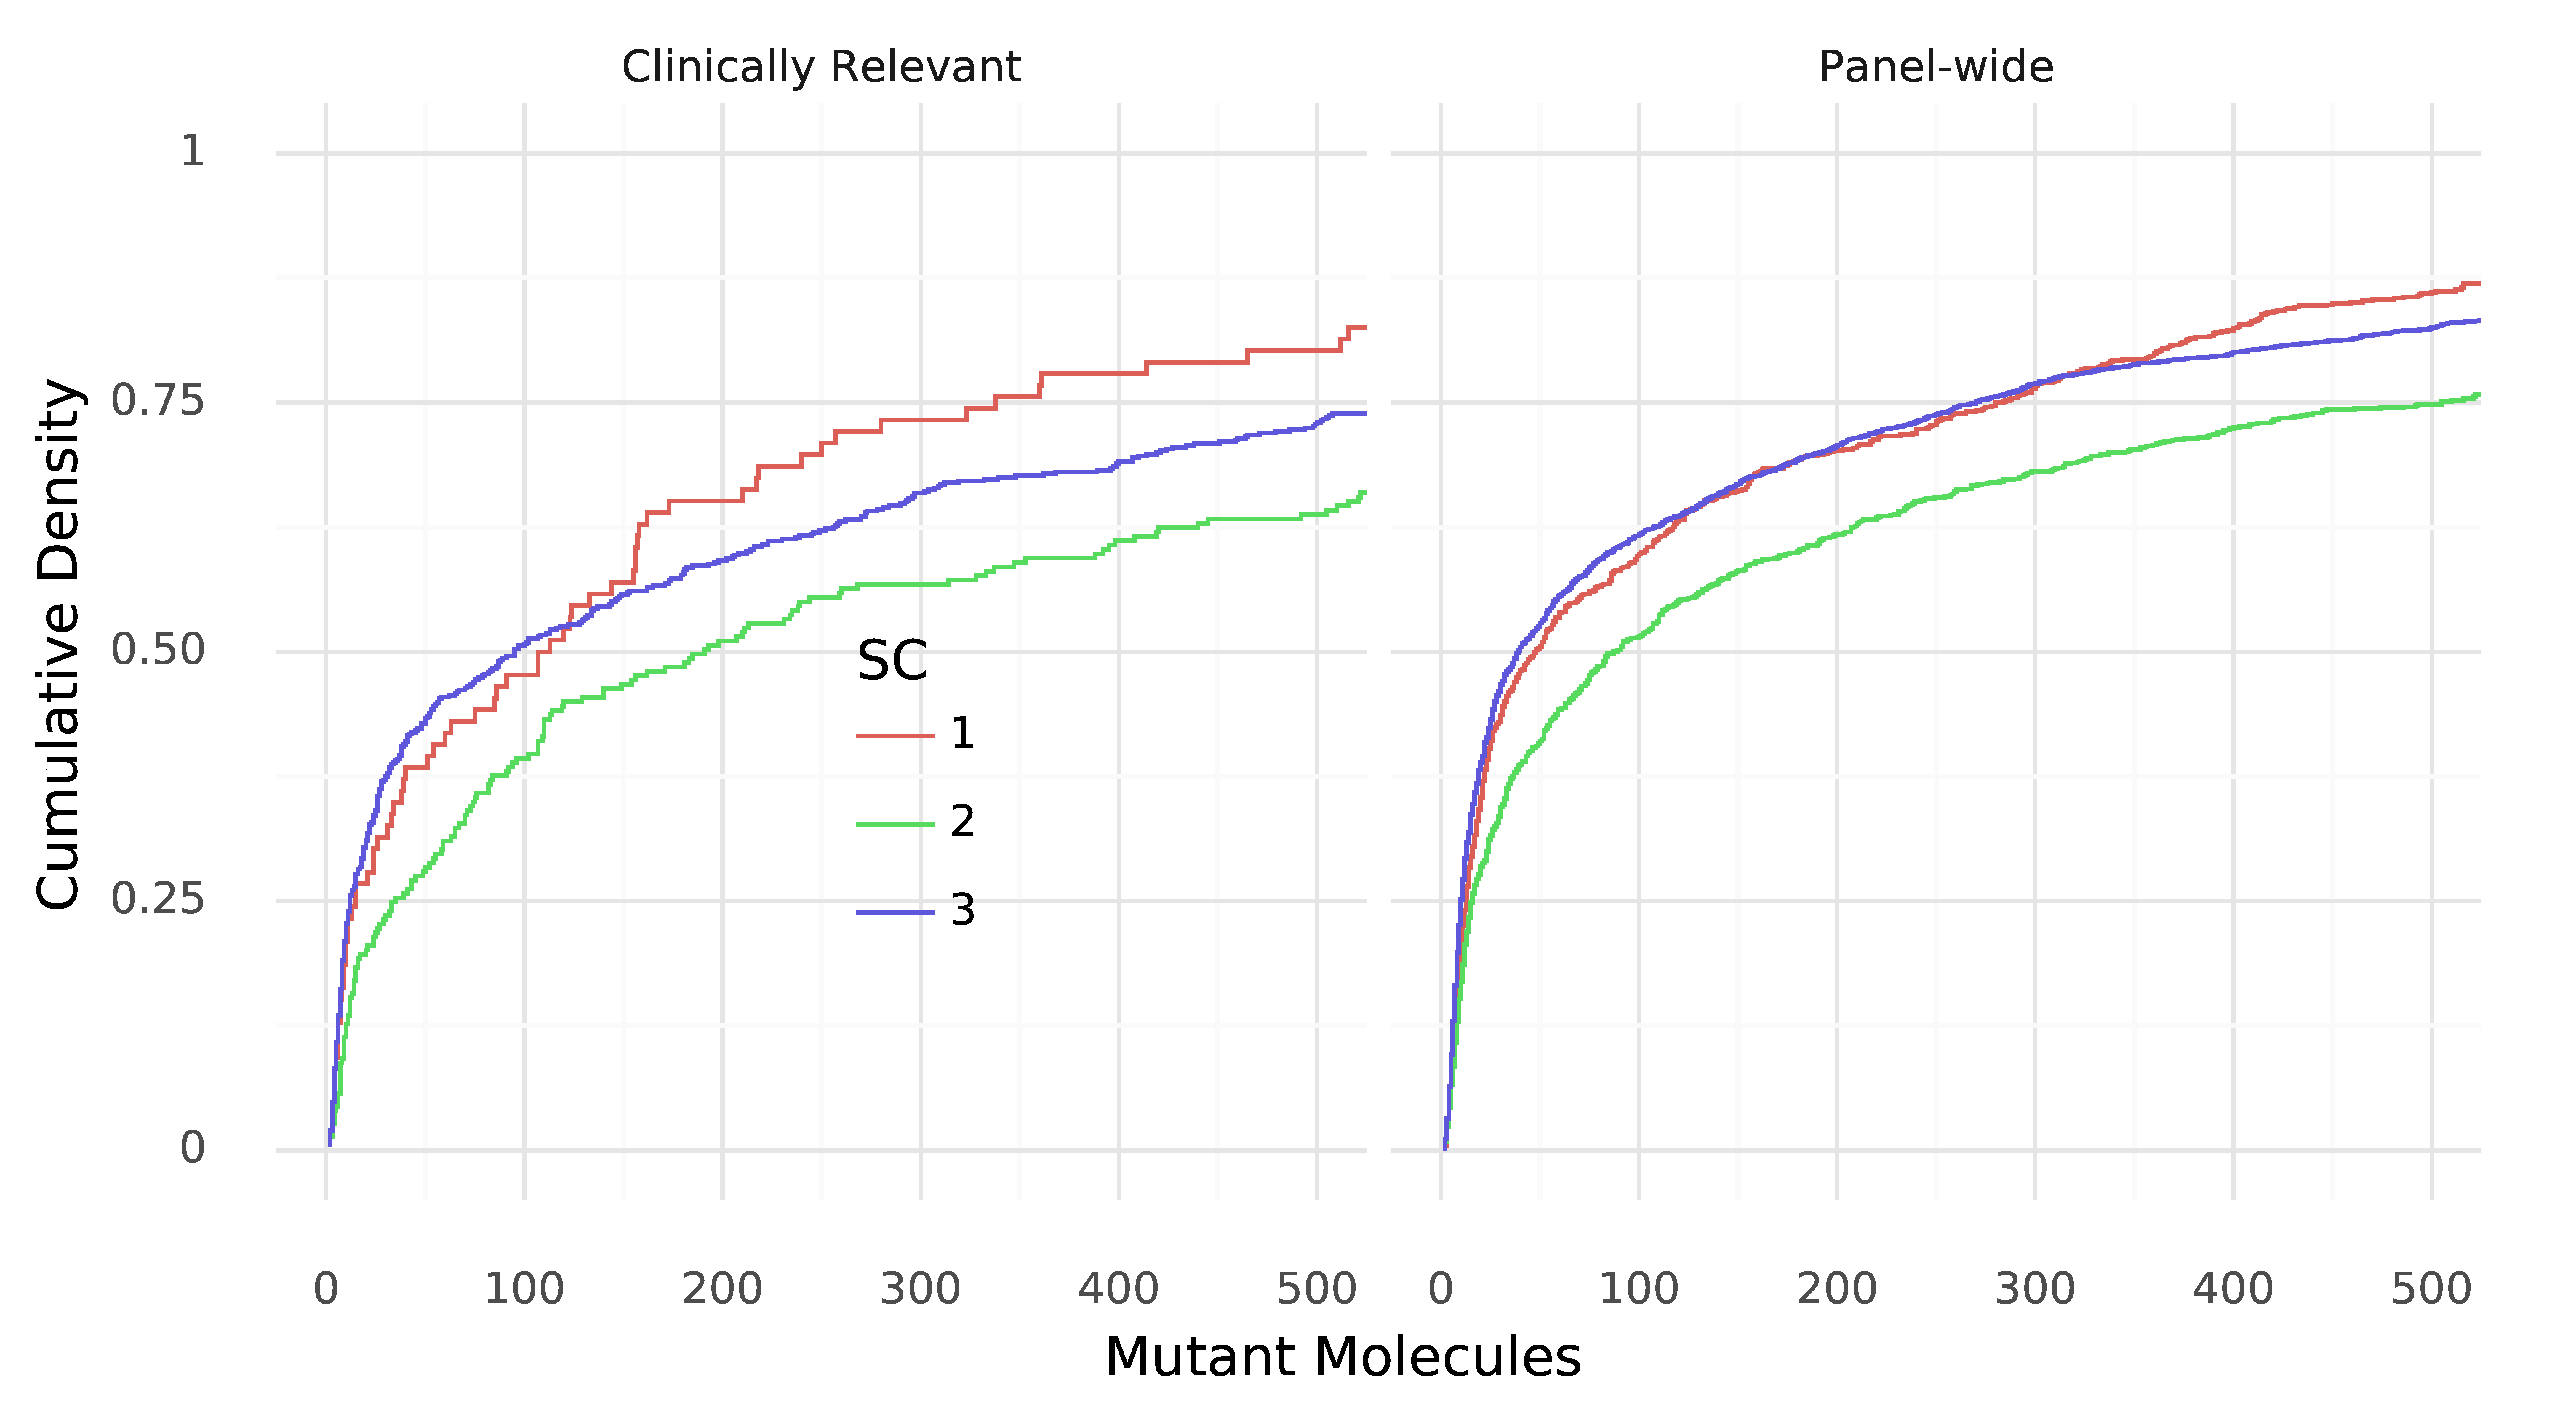
\includegraphics{figures/mol_plot.png}
    \caption{Cumulative densities for mutant molecule counts for each sample collection}
    \label{fig:cdf_molecule_counts}
\end{figure}

\end{appendices}




\end{document}
